% ============================================================================
% RAPPORT DE STAGE — FlexiMax (squelette à compléter)
% ============================================================================
% Mode d'emploi
%  - Deux types de boîtes de guidage, à SUPPRIMER une fois la section rédigée :
%      \begin{todobox}[Source : ...]   -> indique quoi écrire et où trouver
%      l'information (quel notebook, quelle cellule/figure).
%      \begin{figplaceholder}{...}     -> emplacement d'une figure pas encore
%      exportée depuis un notebook.
%  - \begin{resultbox}[...]            -> résultats déjà validés (repris de
%      reports/rapport_modelisation.tex), réutilisables tels quels.
%  - Les figures déjà présentes dans reports/figures/ sont directement
%    incluses avec \includegraphics (clustering, modélisation, RNN/MLP) —
%    seule la légende/l'analyse reste à compléter.
%  - Compilation : pdflatex rapport_stage.tex (x2 pour la table des matières),
%    exécuté depuis le dossier reports/.
%  - Rappel (cf. mémoire projet) : ne t'appuie que sur tes propres notebooks
%    pour extraire les résultats ; ceux de Boubaker restent des références en
%    lecture seule.
% ============================================================================

\documentclass[11pt,a4paper]{report}

\usepackage[french]{babel}
\usepackage[utf8]{inputenc}
\usepackage[T1]{fontenc}
\usepackage{lmodern}
\usepackage{textcomp}
\usepackage{geometry}
\usepackage{booktabs}
\usepackage{array}
\usepackage{xcolor}
\usepackage{tikz}
\usetikzlibrary{arrows.meta,positioning,fit,calc}
\usepackage[most]{tcolorbox}
\usepackage{titlesec}
\usepackage{fancyhdr}
\usepackage{enumitem}
\usepackage{graphicx}
\usepackage{amsmath}
\usepackage{float}
\usepackage{caption}
\usepackage{subcaption}
\usepackage[hidelinks]{hyperref}
\usepackage{alltt}
\usepackage{placeins}
\usepackage{etoolbox}
\usepackage{pdflscape}
\usepackage{colortbl}
\usepackage{pifont}
\usepackage{longtable}

\geometry{margin=2cm}
\graphicspath{{figures/}{../figures/}}

% ---------------------------------------------------------------------------
% Mise en page compacte --- règle valable pour tout le rapport, y compris les
% sections ajoutées par la suite (listes, tableaux, figures, boîtes).
% ---------------------------------------------------------------------------
\setlist{nosep, topsep=3pt, itemsep=2pt, parsep=0pt}
\renewcommand{\arraystretch}{0.92}
\setlength{\abovecaptionskip}{3pt}
\setlength{\belowcaptionskip}{1pt}
\setlength{\intextsep}{4pt plus 1pt minus 1pt}
\setlength{\textfloatsep}{5pt plus 1pt minus 1pt}
\setlength{\floatsep}{4pt plus 1pt minus 1pt}

% Places plus de flottants par page avant de forcer une page dédiée --- limite le nombre de
% pages perdues à attendre qu'un flottant [htbp] trouve sa place idéale.
\setcounter{topnumber}{9}
\setcounter{bottomnumber}{9}
\setcounter{totalnumber}{16}
\renewcommand{\topfraction}{0.9}
\renewcommand{\bottomfraction}{0.9}
\renewcommand{\textfraction}{0.05}
\renewcommand{\floatpagefraction}{0.75}

% ---------------------------------------------------------------------------
% Palette « énergie » FlexiMax
% ---------------------------------------------------------------------------
\definecolor{energydark}{RGB}{18,44,61}      % bleu graphite (structure)
\definecolor{energyaccent}{RGB}{245,166,35}  % ambre (énergie / à compléter)
\definecolor{energygreen}{RGB}{62,158,108}   % vert (résultat validé)
\definecolor{energygrey}{RGB}{107,114,128}   % gris (texte secondaire)

\newcommand{\code}[1]{\texttt{#1}}
\providecommand{\degree}{}
\renewcommand{\degree}{\textdegree}

% ---------------------------------------------------------------------------
% Couleurs et marqueurs --- tableau détaillé des attributs (\S\ref{sec:agregation-physique})
% ---------------------------------------------------------------------------
\definecolor{csocio}{RGB}{255,210,210}
\definecolor{coccup}{RGB}{210,225,255}
\definecolor{cmeteo}{RGB}{210,245,215}
\definecolor{cenvel}{RGB}{255,252,210}
\definecolor{csyste}{RGB}{235,210,255}
\definecolor{cusage}{RGB}{255,228,180}
\definecolor{cblanc}{RGB}{200,245,245}
\definecolor{cagg}{RGB}{200,235,230}
\definecolor{hsocio}{RGB}{210,110,110}
\definecolor{hoccup}{RGB}{100,140,210}
\definecolor{hmeteo}{RGB}{100,185,120}
\definecolor{henvel}{RGB}{200,185,60}
\definecolor{hsyste}{RGB}{160,100,210}
\definecolor{husage}{RGB}{210,155,60}
\definecolor{hblanc}{RGB}{60,185,185}
\definecolor{hagg}{RGB}{40,150,135}

\newcommand{\var}[1]{\texttt{\small #1}}
\newcommand{\Sup}{\textcolor{red!75!black}{\ding{55}~\textbf{\footnotesize supprimé}}}
\newcommand{\Keep}{\textcolor{green!50!black}{\ding{51}~\footnotesize conservé}}
\newcommand{\Newagg}{\textcolor{hagg}{\ding{72}~\textbf{\footnotesize agrégat}}}

% ---------------------------------------------------------------------------
% Boîtes de guidage
% ---------------------------------------------------------------------------
\newtcolorbox{todobox}[1][À compléter]{
  enhanced, breakable,
  colback=energyaccent!8, colframe=energyaccent!85!black,
  coltitle=white, colbacktitle=energyaccent!85!black,
  fonttitle=\bfseries\small, title=#1,
  boxrule=0.5pt, arc=2pt, left=5pt, right=5pt, top=2pt, bottom=2pt,
  before skip=3pt, after skip=4pt
}

\newtcolorbox{resultbox}[1][Résultat déjà disponible]{
  enhanced, breakable,
  colback=energygreen!8, colframe=energygreen!60!black,
  coltitle=white, colbacktitle=energygreen!60!black,
  fonttitle=\bfseries\small, title=#1,
  boxrule=0.5pt, arc=2pt, left=5pt, right=5pt, top=2pt, bottom=2pt,
  before skip=3pt, after skip=4pt
}

\newtcolorbox{figplaceholder}[1][]{
  colback=black!3, colframe=energygrey!70!black,
  boxrule=0.6pt, arc=1pt, halign=center, valign=center,
  height=4cm, fontupper=\itshape\color{energygrey!30!black},
  before skip=4pt, after skip=6pt, #1
}

% ---------------------------------------------------------------------------
% Titres de chapitres / sections
% ---------------------------------------------------------------------------
\titleformat{\chapter}[display]
  {\normalfont\bfseries}
  {\filright\normalsize\color{energygrey}\MakeUppercase{\chaptertitlename}~\thechapter}
  {4pt}
  {\filright\Huge\color{energydark}}
  [\vspace{2pt}{\color{energyaccent}\titlerule[2.2pt]}\vspace{6pt}]

% Force le placement de tous les flottants [htbp] en attente avant chaque nouveau chapitre ---
% évite l'erreur "Float(s) lost" et les pages orphelines de flottants non placés.
\pretocmd{\chapter}{\FloatBarrier}{}{}

\titleformat{\section}
  {\large\bfseries\color{energydark}}{\thesection}{0.6em}{}
  [{\color{energyaccent}\titlerule[1pt]}]
\titleformat{\subsection}
  {\normalsize\bfseries\color{energydark!80!black}}{\thesubsection}{0.6em}{}
\titleformat{\subsubsection}
  {\normalsize\bfseries\itshape\color{energydark!70!black}}{\thesubsubsection}{0.6em}{}

% Espacement resserré autour des titres --- gain cumulé sur ~12 chapitres et ~35 sections.
\titlespacing*{\chapter}{0pt}{0pt}{16pt}
\titlespacing*{\section}{0pt}{10pt}{4pt}
\titlespacing*{\subsection}{0pt}{8pt}{3pt}
\titlespacing*{\subsubsection}{0pt}{6pt}{2pt}

% ---------------------------------------------------------------------------
% En-têtes / pieds de page
% ---------------------------------------------------------------------------
\pagestyle{fancy}
\fancyhf{}
\renewcommand{\headrulewidth}{0.6pt}
\renewcommand{\footrulewidth}{0pt}
\renewcommand{\headrule}{{\color{energyaccent}\hrule height\headrulewidth \vskip-\headrulewidth}}
\fancyhead[L]{\small\color{energygrey}\leftmark}
\fancyhead[R]{\small\color{energygrey}\thepage}
\fancypagestyle{plain}{%
  \fancyhf{}
  \fancyhead[R]{\small\color{energygrey}\thepage}
  \renewcommand{\headrulewidth}{0pt}
}

\hypersetup{
  pdftitle={Rapport de stage - FlexiMax},
  pdfauthor={Yassmin Zouarhi},
  pdfsubject={Prédiction de la consommation énergétique résidentielle - ResStock},
}

\begin{document}

% ============================================================================
% PAGE DE GARDE
% ============================================================================
\begin{titlepage}
\noindent\hspace*{-2cm}%
\begin{tikzpicture}
\useasboundingbox (0,0) rectangle (21cm,8.6cm);
\fill[energydark] (0,0) rectangle (21cm,8.6cm);
\fill[energyaccent] (0,0) rectangle (21cm,0.22cm);
% Icône « éclair énergie »
\begin{scope}[xshift=8.6cm,yshift=6.7cm,scale=1.8]
\fill[energyaccent] (0.55,1.0) -- (0.15,0.35) -- (0.42,0.35) -- (0.20,-0.35)
                     -- (0.85,0.45) -- (0.55,0.45) -- (0.78,1.0) -- cycle;
\end{scope}
\node[white,align=center,font=\Huge\bfseries] at (10.5,4.9) {Rapport de stage};
\node[energyaccent!90!white,align=center,font=\Large\bfseries] at (10.5,3.9)
  {FlexiMax - Flexibilité énergétique résidentielle};
\node[white!85!black,align=center,font=\normalsize] at (10.5,3.1)
  {Prédiction de la consommation énergétique à partir des données ResStock};
\end{tikzpicture}

\vspace{1.4cm}
\begin{center}
{\Large\textbf{MINES Paris - PSL / ARMINES}}\\[2pt]
{\normalsize Programme France 2030 - ADEME}\\[14pt]
{\color{energyaccent}\rule{6cm}{0.8pt}}\\[14pt]
{\large\textbf{Yassmin Zouarhi}}\\[6pt]
\normalsize Stage de \emph{4 mois}, \emph{2025/2026}\\[4pt]
Encadrants : \emph{Gilles Guerassimoff, Damien Corral, Abderrahmane Habbal}\\[24pt]
\today
\end{center}
\vfill
\begin{center}
\includegraphics[height=1.3cm]{logo_polytech.png}\hspace{2cm}%
\includegraphics[height=1.3cm]{logo_mines_psl.png}
\end{center}
\vspace{10pt}

\begin{center}
{\footnotesize\color{energygrey}
Pipeline de notebooks : \code{01\_exploration} $\rightarrow$ \code{02\_nettoyage} $\rightarrow$
\code{03\_visualisation} $\rightarrow$ \code{04\_features} $\rightarrow$ \code{05\_deeplearning}
$\rightarrow$ \code{06\_timeseries} - dépôt \code{FlexiMax}\par}
\end{center}
\end{titlepage}

% ============================================================================
\chapter*{Remerciements}
\addcontentsline{toc}{chapter}{Remerciements}

Je tiens à remercier chaleureusement mes deux tuteurs de stage, Gilles Guerassimoff et
Damien Corral, pour leur suivi régulier, leur disponibilité et leurs conseils tout au
long de ce projet, ainsi que pour la confiance accordée dans la conduite des différentes étapes
de l'analyse.

Je remercie également Abderrahmane Habbal, mon tuteur académique à Polytech, pour
son accompagnement et le suivi pédagogique apporté durant ce stage.

Mes remerciements vont aussi à Didier Auroux, responsable de stage de la
filière MAM à Polytech, pour son suivi et sa disponibilité tout au long
de cette expérience.

Je souhaite aussi remercier l'ensemble de l'équipe du programme FlexiMax à MINES Paris - PSL /
ARMINES pour son accueil et pour les échanges enrichissants sur les enjeux de flexibilité
énergétique résidentielle, ainsi que pour l'accès aux données et aux outils nécessaires à la
réalisation de ce travail.

Merci également à Boubaker Amdyoun, avec qui j'ai partagé ce dépôt de travail, pour les échanges
techniques et méthodologiques qui ont permis d'améliorer la fiabilité des analyses présentées
dans ce rapport.

Je remercie aussi Eyua Assoumou, stagiaire ayant rejoint l'équipe pour un mois, qui nous a aidés à
lancer l'exploration des séries temporelles.

Enfin, je remercie le programme France 2030 et l'ADEME pour le financement de ce projet de
recherche.

% ============================================================================
\chapter*{Résumé}
\addcontentsline{toc}{chapter}{Résumé}

Combien d'électricité un bâtiment résidentiel va-t-il consommer, et pourquoi ? Ce
stage, mené dans le cadre du programme FlexiMax (MINES Paris - PSL / ARMINES, France 2030 /
ADEME), construit pas à pas une chaîne de modélisation de la consommation énergétique
résidentielle. En l'absence de données disponibles sur le projet FlexiMax lui-même au moment du
stage, ce travail s'appuie sur un cas d'étude alternatif : les données de simulation ResStock
(NREL) - près de 550\,000 bâtiments, chacun décrit par plusieurs centaines de variables et une
série temporelle horaire sur un an.

L'exploration révèle que, sous les 771 colonnes brutes du jeu de métadonnées, se cachent des
doublons et artefacts de simulation (391 colonnes retenues) ; un même facteur revient sans cesse,
la zone climatique. Elle structure la consommation de chauffage/climatisation, borne le
potentiel de flexibilité des thermostats (43,8\,\% seulement des bâtiments disposent d'un
thermostat programmable pour le chauffage), et réapparaîtra comme déterminant n°1 du modèle
prédictif final. Ce fil conducteur, la géographie climatique comme clé de lecture de la
consommation, traverse tout le rapport, de l'exploration au clustering des profils
journaliers jusqu'à l'importance des variables du modèle LightGBM.

Pour la cohérence du périmètre, l'analyse se recentre ensuite sur les bâtiments
\textbf{tout-électriques}. Un pipeline de feature engineering réduit 108 attributs bruts à 83
features physiquement interprétables, dont cinq agrégats d'enveloppe qui remplacent une trentaine
de variables catégorielles propres au parc états-unien. Un modèle LightGBM entraîné sur ce
périmètre atteint un $R^2$ de 0,925 sur la consommation électrique - contre 0,845 avant le
recentrage tout-électrique - avec un écart minime face au jeu de features réduit aux seuls
agrégats physiques. Le clustering des profils journaliers révèle ensuite des « jours types »
récurrents, à l'échelle d'un bâtiment puis d'un panel de 100 logements, avant qu'une architecture
hybride RNN/MLP n'explore deux horizons de prédiction sur les séries horaires : prévoir la
consommation à l'heure suivante ($R^2=0{,}877$) et extrapoler la consommation annuelle à partir de
90 jours d'observation ($R^2=0{,}803$).

Le rapport livre ainsi moins une collection de modèles qu'une lecture cohérente des déterminants
de la consommation électrique résidentielle, et une chaîne reproductible pour l'étendre.

\section*{Abstract}

How much electricity will a residential building draw, and why? This internship, carried out within the
FlexiMax program (MINES Paris - PSL / ARMINES, France 2030 / ADEME), builds step by step a
residential energy consumption modelling pipeline. With no data yet available on the FlexiMax
project itself at the time of the internship, this work relies on an alternative case study:
the ResStock simulation dataset (NREL) - close to 550,000 buildings, each described by hundreds
of attributes and a full year of hourly time series.

Exploration shows that behind the 771 raw metadata columns lie duplicates and simulation
artifacts (391 columns retained); one factor keeps resurfacing, the climate zone. It shapes
heating/cooling consumption, bounds thermostat flexibility potential (only 43.8\% of buildings
have a programmable heating thermostat), and later re-emerges as the top determinant of the
final predictive model. This thread, climate geography as the key to reading consumption, 
runs through the report, from metadata exploration to daily-profile clustering to LightGBM
feature importance.

For scope coherence, the analysis then focuses on \textbf{all-electric} buildings. A feature
engineering pipeline reduces 108 raw attributes to 83 physically interpretable features, including
five envelope aggregates that replace about thirty categorical variables specific to the US
housing stock. A LightGBM model trained on this scope reaches an $R^2$ of 0.925 on electricity
consumption, versus 0.845 before the all-electric recentering, with only a small gap versus
the feature set reduced to the physical aggregates alone. Clustering the daily profiles then
reveals recurring "typical days", at the scale of a single building and of a 100-building panel,
before a hybrid RNN/MLP architecture tackles two prediction horizons on the hourly series:
forecasting next-hour consumption ($R^2=0.877$) and extrapolating annual consumption from 90 days
of observation ($R^2=0.803$).

The report thus delivers less a collection of models than a coherent reading of what drives
residential electricity consumption, and a reproducible pipeline to extend it.

\enlargethispage{2\baselineskip}
\tableofcontents
\listoffigures
\listoftables
% ============================================================================
\chapter{Contexte : le stage, FlexiMax et les données}
\label{ch:contexte}

\section{Le jeu de données ResStock}
\label{sec:jeu-donnees-resstock}
Le jeu de données central de ce stage est \textbf{ResStock 2025 Release 1}, produit par le
National Renewable Energy Laboratory (NREL) : une simulation bâtiment par bâtiment du parc
résidentiel américain, à partir de modèles EnergyPlus calibrés sur le parc réel (recensement,
enquêtes RECS). Le fichier national \code{upgrade0.parquet} - scénario \emph{baseline}, avant
upgrades - couvre 549\,971 bâtiments décrits par 771 colonnes.

Ces colonnes se répartissent en deux familles, une distinction qui structure tout le rapport :
\begin{itemize}
  \item les variables \textbf{\code{in.*}} (« inputs ») décrivent le bâtiment simulé :
  localisation, géométrie, enveloppe thermique, système HVAC, appareils, profil socio-économique
, ce sont les \emph{features} des modèles prédictifs ;
  \item les variables \textbf{\code{out.*}} (« outputs ») sont les résultats de simulation
  EnergyPlus : consommations par usage et vecteur énergétique (électricité, gaz naturel, propane,
  fioul), émissions de CO$_2$e, factures, dimensionnement, heures d'inconfort... Elles fournissent
  les \emph{cibles} des modèles (\code{out.electricity.total.energy\_consumption..kwh} pour la
  consommation électrique annuelle) et plusieurs indicateurs de lecture (décomposition par usage,
  cf. \S\ref{sec:visual-national}).
\end{itemize}

\begin{resultbox}[Répartition \code{in.*} / \code{out.*} - Source : \code{02\_nettoyage/nettoyage\_metadata.ipynb}]
Après nettoyage (\S\ref{sec:nettoyage-metadata}), les 391 colonnes se répartissent en 165
\code{in.*}, 221 \code{out.*} et 5 colonnes d'identification/pondération.
\begin{table}[H]
\centering
\caption{Structure du jeu de métadonnées nettoyé (391 colonnes, 549\,971 bâtiments).}
\begin{tabular}{lr}
\toprule
Famille & Colonnes \\
\midrule
\code{in.*} - caractéristiques du bâtiment (features)          & 165 \\
\code{out.*} - résultats de simulation (cibles \& indicateurs) & 221 \\
Identifiants et pondération (\code{bldg\_id}, \code{weight}...)  & 5 \\
\bottomrule
\end{tabular}
\end{table}
Ce ratio out/in (1,3 sortie par entrée) reflète la richesse des sorties EnergyPlus
(décomposition fine par usage et vecteur) face à des entrées plus synthétiques : la difficulté
du problème de prédiction ne vient donc pas d'un manque de cibles, mais du choix de la bonne
cible parmi les \code{out.*} et des bonnes \emph{features} parmi les \code{in.*}.
\end{resultbox}

Deux autres sources complètent le jeu ResStock : les séries temporelles individuelles par
bâtiment (pas 15~minutes, 35\,040 lignes/an, téléchargées depuis l'OEDI via
\code{extraction\_timeseries\_oedi.ipynb}) et les données météo horaires par zone climatique
ASHRAE utilisées par EnergyPlus. Le guide technique ResStock
(\code{ResStockTechnicalReferenceGuide\_2025\_1.pdf}, dans \code{reports/figures/}) documente la
définition exacte de chaque variable citée dans ce rapport.

\textbf{Un choix méthodologique à expliciter :} FlexiMax est un projet français (MINES Paris -
PSL / ARMINES, France 2030 / ADEME), mais aucune base résidentielle française de résolution
et de richesse comparable à ResStock n'était disponible pour ce stage, d'où le recours aux
données américaines du NREL. Ce choix n'est pas neutre : le parc américain diffère du parc
français sur plusieurs dimensions rencontrées au fil de l'analyse - le mix énergétique du
chauffage (part du gaz et du fioul bien plus importante aux États-Unis qu'en France), les
habitudes de vie et d'occupation, la mobilité (le
véhicule électrique et son infrastructure de recharge sont modélisés selon des usages
nord-américains) et le parc d'équipements électroménagers (types, tailles, rendements). Les
résultats de ce rapport décrivent donc le parc résidentiel \emph{américain} ; leur transposition
au contexte français reste à valider dès que des données comparables seront disponibles.

\section{Nettoyage des métadonnées}
\label{sec:nettoyage-metadata}
Avant toute exploration, encore faut-il s'assurer que les 771 colonnes brutes sont exploitables :
\begin{resultbox}[Source : \code{02\_nettoyage/nettoyage\_metadata.ipynb}]
Le fichier national brut (\code{upgrade0.parquet}) contient 549\,971 bâtiments $\times$ 771
colonnes. 380 colonnes sont supprimées selon 6 critères, pour 391 colonnes conservées :
\begin{itemize}
  \item \code{upgrade.*} (20 col.) - toutes vides dans le scénario baseline (\code{upgrade=0}) ;
  \item \code{calc.weighted.*} (172 col.) - agrégats de pondération, non utiles bâtiment par
  bâtiment ;
  \item \code{out.*} \emph{savings/reduction} (164 col.) - économies vs upgrade, toutes à 0 en
  baseline ;
  \item \code{in.simulation\_control.*} (6 col.) - identiques pour tous les bâtiments ;
  \item \code{in.utility\_bill.*} (8 col.) - déjà présentes sous \code{out.utility\_bills.*} ;
  \item doublons de colonnes « binned » moins précises que leur équivalent continu (10 col.).
\end{itemize}
Après nettoyage : 0 colonne entièrement vide, 0 colonne à plus de 50\% de valeurs manquantes.
Ces suppressions ne traduisent pas un problème de qualité (aucune donnée aberrante ou incomplète)
mais des artefacts de la méthodologie ResStock elle-même (répétition du scénario \emph{baseline}
dans les colonnes \code{upgrade.*}/\emph{savings}, doublons d'agrégation) : le jeu nettoyé,
exporté vers \code{data/processed/metadata\_clean.parquet}, est donc directement exploitable
sans étape d'imputation.
\end{resultbox}

\begin{figure}[htbp]
  \centering
  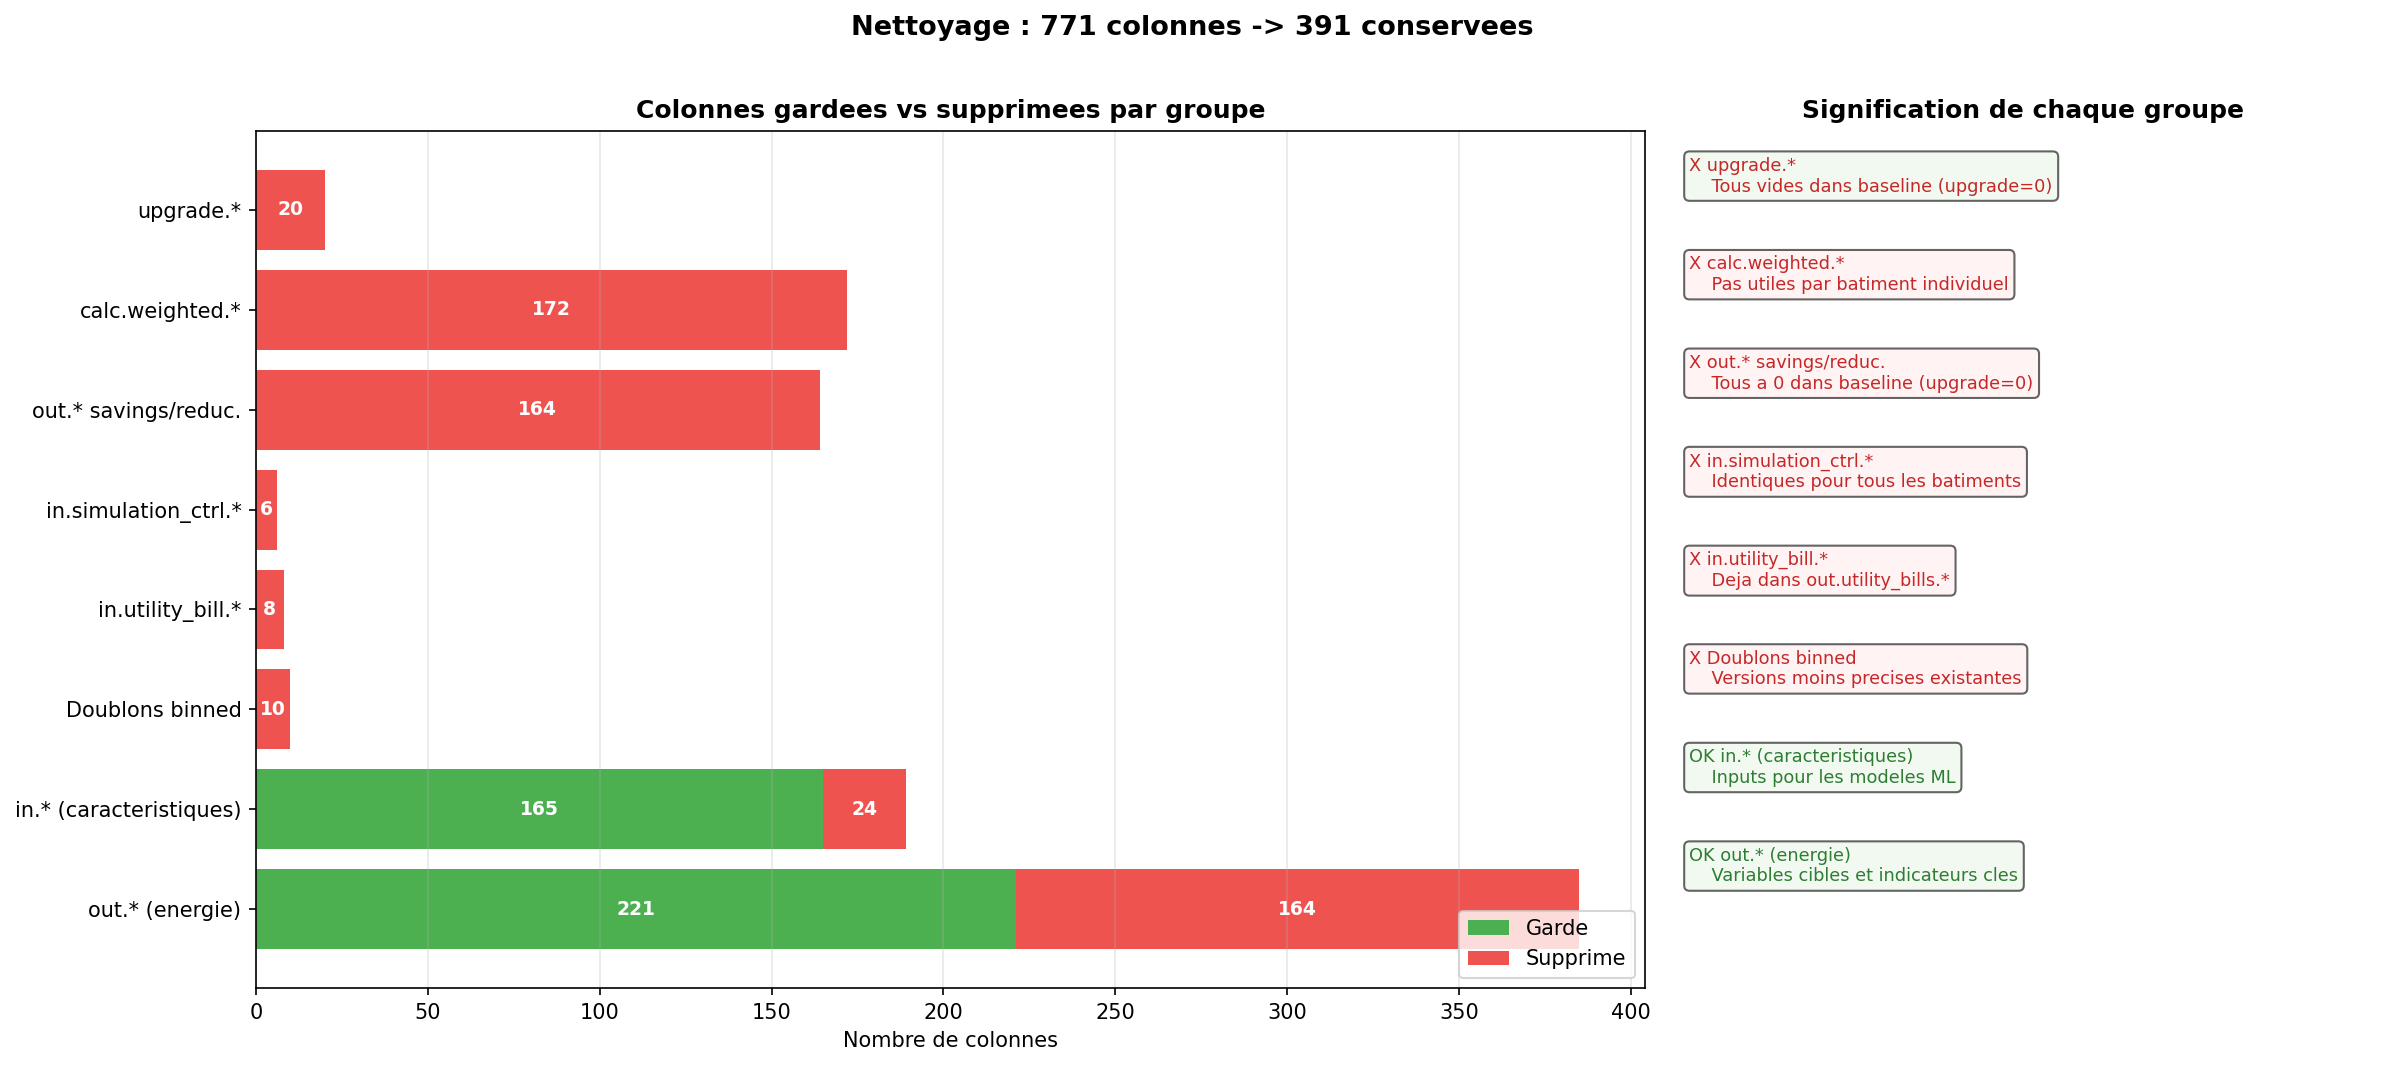
\includegraphics[width=0.8\textwidth]{diagramme_nettoyage.png}
  \caption{Colonnes gardées vs supprimées par groupe (771 $\to$ 391 colonnes).}
  \label{fig:nettoyage-diagramme}
\end{figure}

\section{Structure du jeu nettoyé : variables \code{in.*} et \code{out.*}}

\subsection{Variables \code{in.*}}
\begin{resultbox}[Source : \code{01\_exploration/exploration\_in\_groups.ipynb}]
Sur les 391 colonnes du jeu de métadonnées nettoyé, 165 colonnes \code{in.*} décrivent le
bâtiment et ses occupants, réparties en 11 groupes métier (164 colonnes couvertes, seule
\code{in.upgrade\_name} reste hors groupe) :
\begin{table}[H]
\centering
\caption{Les 11 groupes de variables \code{in.*} (549\,971 bâtiments).}
\label{tab:groupes-in}
\begin{tabular}{lrr}
\toprule
Groupe & Colonnes & \% manquant moyen \\
\midrule
Localisation          & 21 & 0,0\% \\
Zone climatique        & 5 & 0,0\% \\
Géométrie du bâtiment  & 20 & 0,0\% \\
Enveloppe thermique    & 17 & 0,0\% \\
HVAC                    & 42 & 0,0\% \\
Eau chaude               & 6 & 0,0\% \\
Appareils électroménagers & 28 & 0,0\% \\
Véhicule électrique      & 6 & 0,0\% \\
Panneau électrique       & 2 & 0,0\% \\
Solaire et stockage      & 4 & 0,0\% \\
Occupants et socio-économique & 13 & 0,9\% \\
\bottomrule
\end{tabular}
\end{table}
Le taux de manquant quasi nul (base \emph{simulée}, pas de non-réponse d'enquête, seul le groupe
Occupants en présente 0,9\%) évite tout travail d'imputation, un confort rare face à des
données réelles de consommation. La richesse du groupe HVAC (42 variables) en fait le principal
réservoir de leviers de flexibilité pilotables (thermostats, systèmes), là où enveloppe et
géométrie (17+20 variables) ne décrivent que des caractéristiques figées du bâti.
\end{resultbox}

\subsection{Variables \code{out.*}}
\begin{resultbox}[Source : \code{02\_nettoyage/nettoyage\_metadata.ipynb} - calcul direct sur \code{metadata\_clean.parquet}]
Les 221 colonnes \code{out.*} sont les résultats de simulation EnergyPlus, réparties en 14
groupes, dominés par la consommation électrique (60 col.) et les paramètres physiques dérivés du
bâtiment (57 col. - surfaces, dimensionnement, contraintes de panneau électrique) :
\begin{table}[H]
\centering
\caption{Les 14 groupes de variables \code{out.*} (549\,971 bâtiments).}
\label{tab:groupes-out}
\begin{tabular}{lrr}
\toprule
Groupe & Colonnes & \% manquant moyen \\
\midrule
Consommation électrique (\code{electricity})       & 60 & 0,0\% \\
Paramètres physiques dérivés (\code{params})         & 57 & 0,0\% \\
Émissions CO$_2$e (\code{emissions})                  & 33 & 0,3\% \\
Consommation gaz naturel (\code{natural\_gas})       & 22 & 0,0\% \\
Consommation propane (\code{propane})                 & 12 & 0,0\% \\
Consommation fioul (\code{fuel\_oil})                  & 8 & 0,0\% \\
Charges thermiques (\code{load})                        & 7 & 0,0\% \\
Factures (\code{utility\_bills})                          & 5 & 0,0\% \\
Eau chaude, volumes (\code{hot\_water})                 & 4 & 0,0\% \\
Énergie totale du site (\code{site\_energy})            & 4 & 0,0\% \\
Puissances dimensionnantes (\code{capacity})            & 3 & 0,0\% \\
Heures d'inconfort thermique (\code{unmet\_hours})     & 3 & 0,0\% \\
Indicateurs de qualité (\code{qoi})                       & 2 & 0,0\% \\
Taux d'effort énergétique (\code{energy\_burden})    & 1 & 12,1\% \\
\bottomrule
\end{tabular}
\end{table}
Seule \code{out.energy\_burden..percentage} présente un manquant notable (12,1\%, probablement
logements vacants ou sans revenu déclaré). Cinq cibles candidates ressortent de ces 221 colonnes,
la consommation totale par vecteur énergétique et les émissions associées, mais chaque
vecteur a sa propre distribution et ses propres facteurs explicatifs : c'est cette hétérogénéité
qui a justifié de n'en retenir qu'une seule, l'électricité, comme cible finale du rapport.
\end{resultbox}

Le jeu de données posé, l'exploration qui suit cherche à identifier lesquelles de ces 165
variables \code{in.*} pèsent réellement sur la consommation, en partant du facteur le plus
immédiat, la géographie, avant d'élargir progressivement aux caractéristiques du bâtiment
lui-même (chapitre~\ref{ch:beyond-climate}).

% ============================================================================
\chapter{Le climat, premier déterminant de la consommation}
\label{ch:exploration}

\section{Localisation et zone climatique}
\label{sec:localisation-climat}
\begin{resultbox}[Source : \code{exploration\_localisation\_climat.ipynb}]
La Californie, le Texas et la Floride concentrent le plus de bâtiments simulés, mais ce sont des
états au climat plus doux (CA en particulier) qui affichent les consommations moyennes les
\emph{plus faibles} du top 20 (8\,030~kWh/an) - à l'inverse, le Tennessee (15\,887~kWh/an), la
Virginie et le Missouri dominent malgré un parc plus petit. Au niveau régional, le Sud regroupe
le plus de bâtiments (210\,283) et la consommation moyenne la plus élevée ($\sim$14\,400~kWh/an) ;
le Nord-Est est la région la moins consommatrice.
\end{resultbox}

\begin{figure}[htbp]
  \centering
  \includegraphics[width=0.8\textwidth]{localisation_etats_conso.png}
  \caption{Top 20 états par nombre de bâtiments et par consommation électrique moyenne ;
  consommation moyenne par région Census.}
  \label{fig:localisation-etats}
\end{figure}

\begin{figure}[htbp]
  \centering
  \includegraphics[width=0.75\textwidth]{localisation_carte_batiments.png}
  \caption{Nombre de bâtiments simulés par état (ResStock).}
  \label{fig:localisation-carte}
\end{figure}

Le nombre de bâtiments simulés ne suit donc pas la consommation : c'est la zone climatique, pas
la taille du parc, qui structure ces écarts.

\begin{resultbox}[Zone climatique ASHRAE - déterminant n°1 identifié par le modèle prédictif]
Les zones 5A (123\,952 bâtiments) et 4A (118\,416) dominent le parc ; les zones extrêmes (1A «
très chaud », 7B/8AK « arctique ») sont marginales ($<$1\,000 bâtiments). Le gradient
chauffage/climatisation est net : la 2B très chaude/humide consomme $\sim$6\,800~kWh/an de
climatisation contre quasiment rien en chauffage, l'inverse pour les zones froides 6A/7A. Le
panneau « pics de puissance été/hiver », lu comme indicateur de \textbf{flexibilité FlexiMax},
montre des pics hivernaux nettement supérieurs aux pics estivaux pour les zones froides (2A,
3A), et l'inverse pour les zones chaudes (1A, 2B) : le potentiel de flexibilité n'est donc pas
uniforme sur le territoire.
\end{resultbox}

\begin{figure}[htbp]
  \centering
  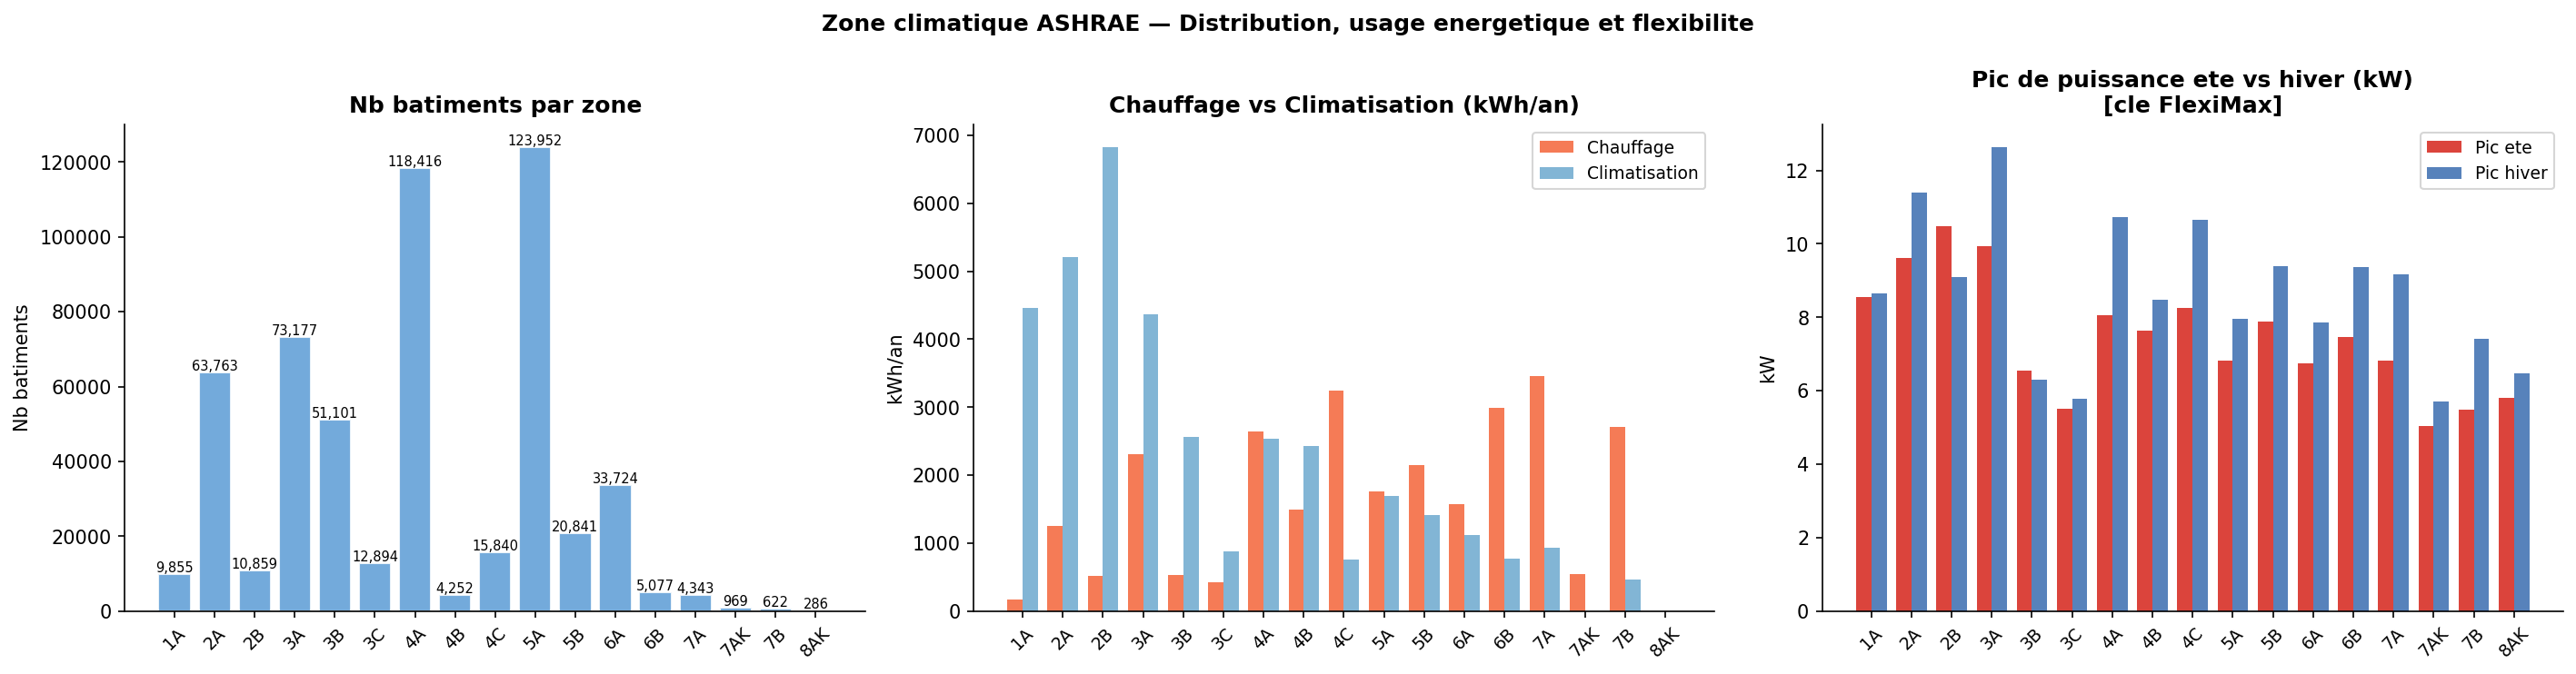
\includegraphics[width=0.82\textwidth]{zones_climatiques_synthese.png}
  \caption{Zones climatiques ASHRAE  -  distribution, usage chauffage/climatisation et pics de
  puissance été/hiver (indicateur de flexibilité FlexiMax).}
  \label{fig:zones-synthese}
\end{figure}

\begin{figure}[htbp]
  \centering
  \includegraphics[width=0.75\textwidth]{zones_climatiques_carte_dominante.png}
  \caption{Zone climatique ASHRAE dominante par état.}
  \label{fig:zones-carte}
\end{figure}

\section{Une dispersion que le climat seul n'explique pas}
\label{sec:dispersion-intra-zone}
Les moyennes par zone (\S\ref{sec:localisation-climat}) masquent la distribution complète : est-ce
que deux bâtiments de la même zone climatique consomment vraiment de façon comparable ?
\begin{resultbox}[Source : \code{visualisation\_metadata.ipynb} - échantillon illustratif de 5\,000 bâtiments]
Vue complémentaire, en distribution complète plutôt qu'en moyenne, de la consommation électrique
par zone climatique : les zones les plus peuplées (4A, 5A) présentent aussi la plus grande
dispersion et les valeurs extrêmes les plus hautes (jusqu'à $\sim$90\,000~kWh/an en zone 7A), ce
que les moyennes seules (\S\ref{sec:localisation-climat}) ne laissaient pas apparaître. Cette
dispersion intra-zone confirme que la zone climatique, quoique déterminante, n'explique pas tout
: d'autres facteurs bâtimentaires et comportementaux restent nécessaires pour capturer les
extrêmes.
\end{resultbox}

\begin{figure}[H]
  \centering
  \includegraphics[width=0.55\textwidth]{visualisation_conso_par_zone_boxplot.png}
  \caption{Distribution (boxplot) de la consommation électrique totale par zone climatique
  ASHRAE, échantillon de 5\,000 bâtiments.}
  \label{fig:vismeta-boxplot}
\end{figure}

Reste donc à identifier ce qui, à zone climatique égale, distingue un bâtiment qui consomme peu
d'un bâtiment qui consomme beaucoup : le bâti, les systèmes techniques et le comportement des
occupants, explorés au chapitre~\ref{ch:beyond-climate}.

% ============================================================================
\chapter{Au-delà du climat : bâti, équipements et comportement}
\label{ch:beyond-climate}

Ce chapitre couvre les trois familles de déterminants encore non explorées - l'enveloppe
thermique, les systèmes techniques (HVAC, eau chaude), et le profil des occupants - avant de les
synthétiser en une classification métier et une lecture par usage et par vecteur énergétique.

\section{Enveloppe thermique}
\begin{resultbox}[Source : \code{exploration\_enveloppe\_thermique.ipynb}]
Pour le plafond et la toiture, la relation isolation $\to$ consommation suit la logique
attendue : la consommation moyenne diminue quand le R-value augmente (plafond non isolé
$\approx$16\,500~kWh vs R-49 $\approx$13\,200~kWh). Pour les murs en revanche, la relation n'est
\emph{pas} monotone (R-15 associé à une consommation plus élevée que R-11 ou R-19) : signe
probable d'un facteur de confusion non contrôlé (l'isolation des murs est corrélée à la zone
climatique et au type de bâtiment). Une lecture « toutes choses égales par ailleurs »
nécessiterait de contrôler ces facteurs (régression multivariée, comparaison à zone climatique
fixée).
\end{resultbox}

\begin{figure}[htbp]
  \centering
  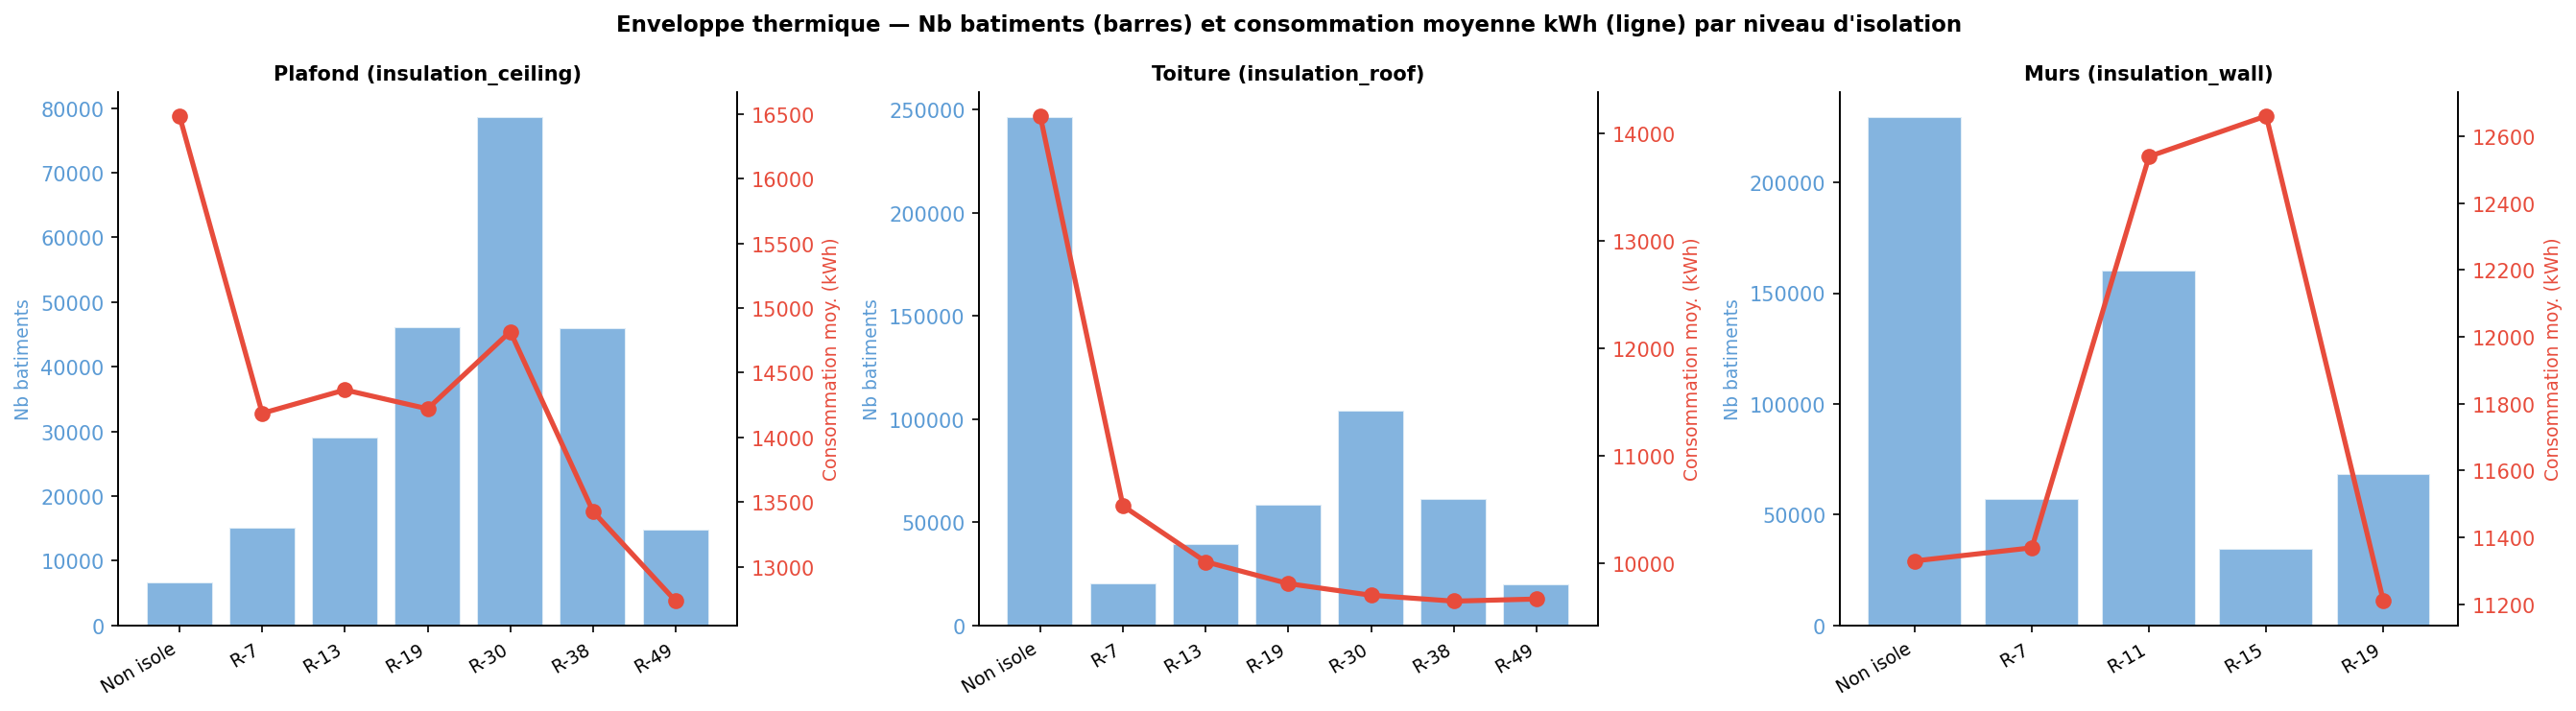
\includegraphics[width=0.82\textwidth]{enveloppe_r_values.png}
  \caption{Nombre de bâtiments et consommation moyenne par niveau d'isolation (R-value),
  plafond / toiture / murs.}
  \label{fig:enveloppe-rvalues}
\end{figure}

\section{Système HVAC}
\begin{resultbox}[Source : \code{exploration\_hvac.ipynb}]
\textbf{Types de systèmes.} La pompe à chaleur gainée (\emph{Ducted Heat Pump}) affiche la
consommation électrique moyenne la plus élevée (15\,845~kWh/an), devant le chauffage gainé
classique (11\,458) et non gainé (9\,847). Côté climatisation, le \emph{Central AC} domine en
nombre (291\,239 bâtiments) devant le \emph{Room AC} (108\,992). Par combustible, le chauffage
électrique a la consommation électrique moyenne la plus élevée (15\,564~kWh/an), loin devant
gaz/propane/fioul ($\sim$9\,000~kWh/an).

\textbf{Consignes de température (flexibilité FlexiMax).} Consigne médiane 70\degree F
(chauffage), 72\degree F (climatisation). \textbf{43,8\%} des bâtiments ont un thermostat
programmable pour le chauffage, \textbf{35,8\%} pour la climatisation : une majorité n'a donc
\emph{pas} de pilotage automatique, ce qui borne le potentiel de flexibilité activable sans
changement d'équipement.

\textbf{Gaines (ducts).} 423\,599 bâtiments sur \(\sim\)550\,000 ont des gaines de distribution
d'air, avec une consommation moyenne nettement supérieure (12\,772~kWh/an) à ceux qui n'en ont
pas (8\,348~kWh/an) - surtout un effet de taille/type de système (gaines associées aux systèmes
centraux, plus consommateurs). Les fuites de gaines sont associées à une surconsommation
croissante avec le taux de fuite, à isolation égale.
\end{resultbox}

\begin{figure}[htbp]
  \centering
  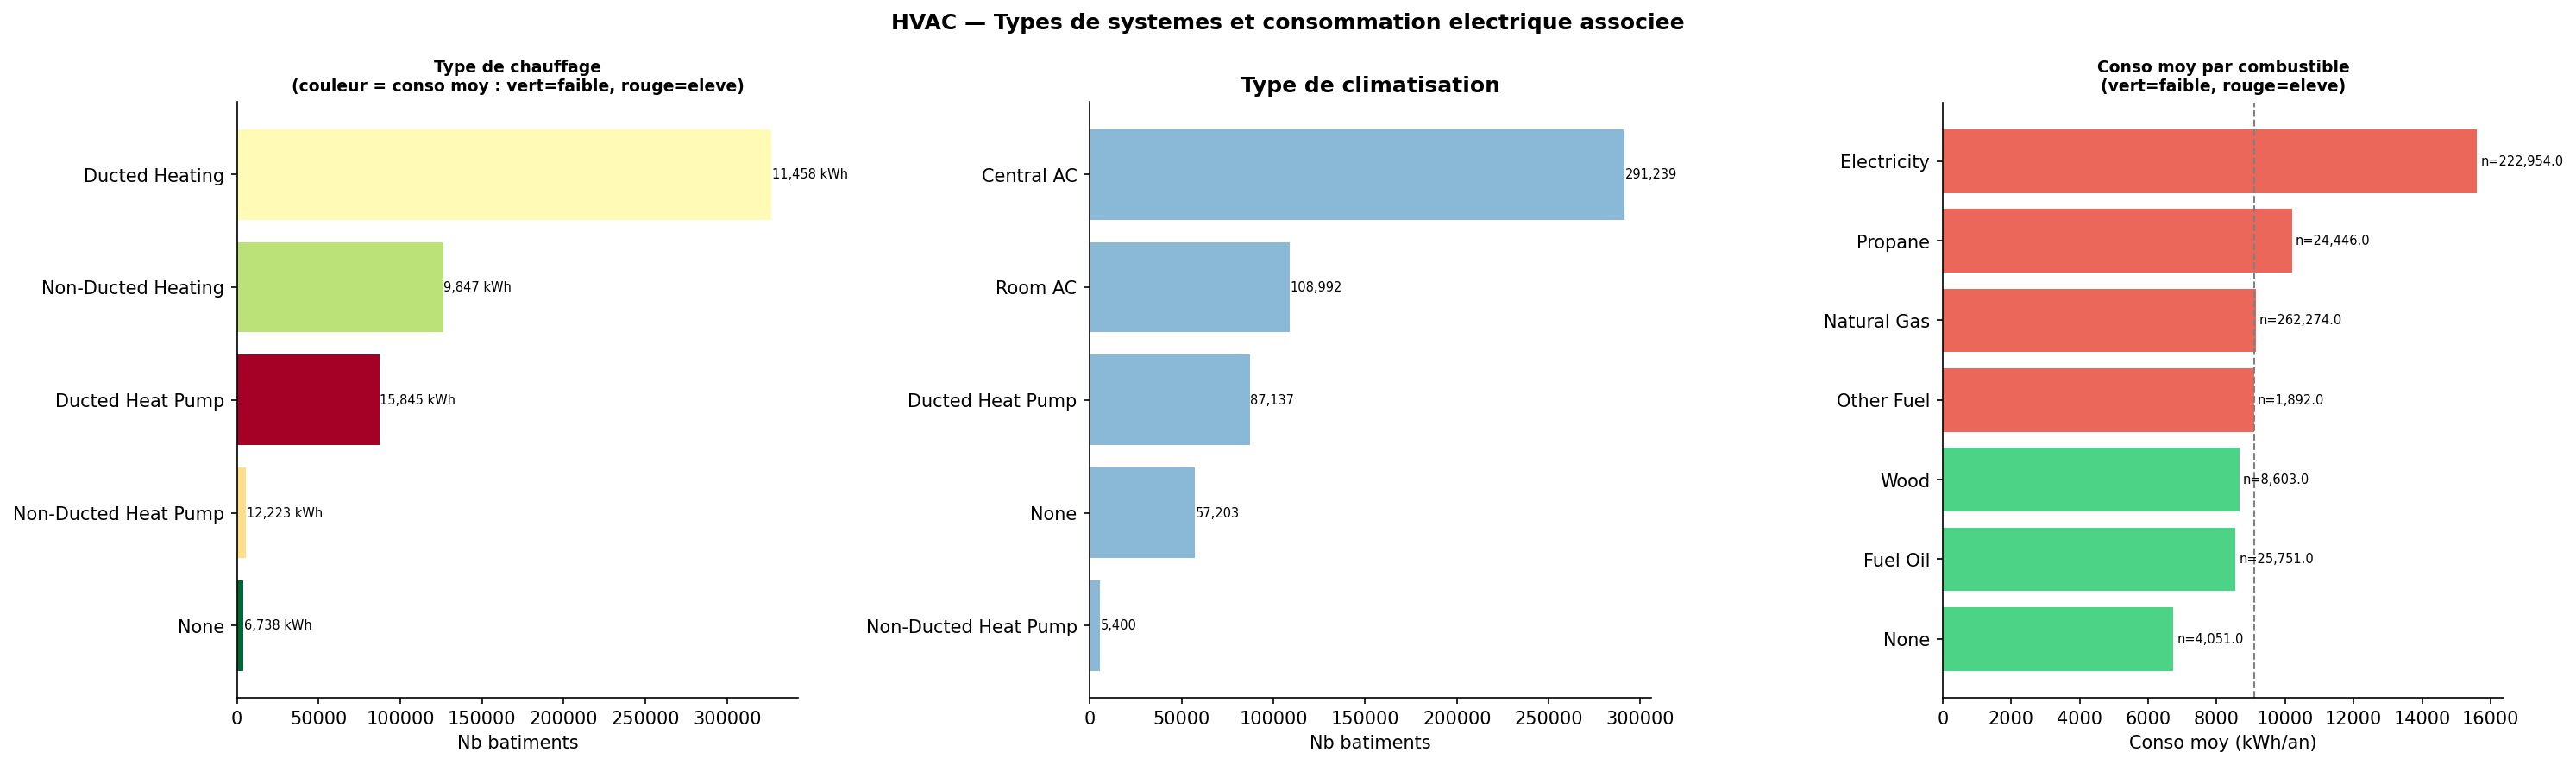
\includegraphics[width=0.82\textwidth]{hvac_types_systemes.png}
  \caption{Types de chauffage/climatisation et consommation associée ; consommation moyenne par
  combustible de chauffage.}
  \label{fig:hvac-types}
\end{figure}

\begin{figure}[htbp]
  \centering
  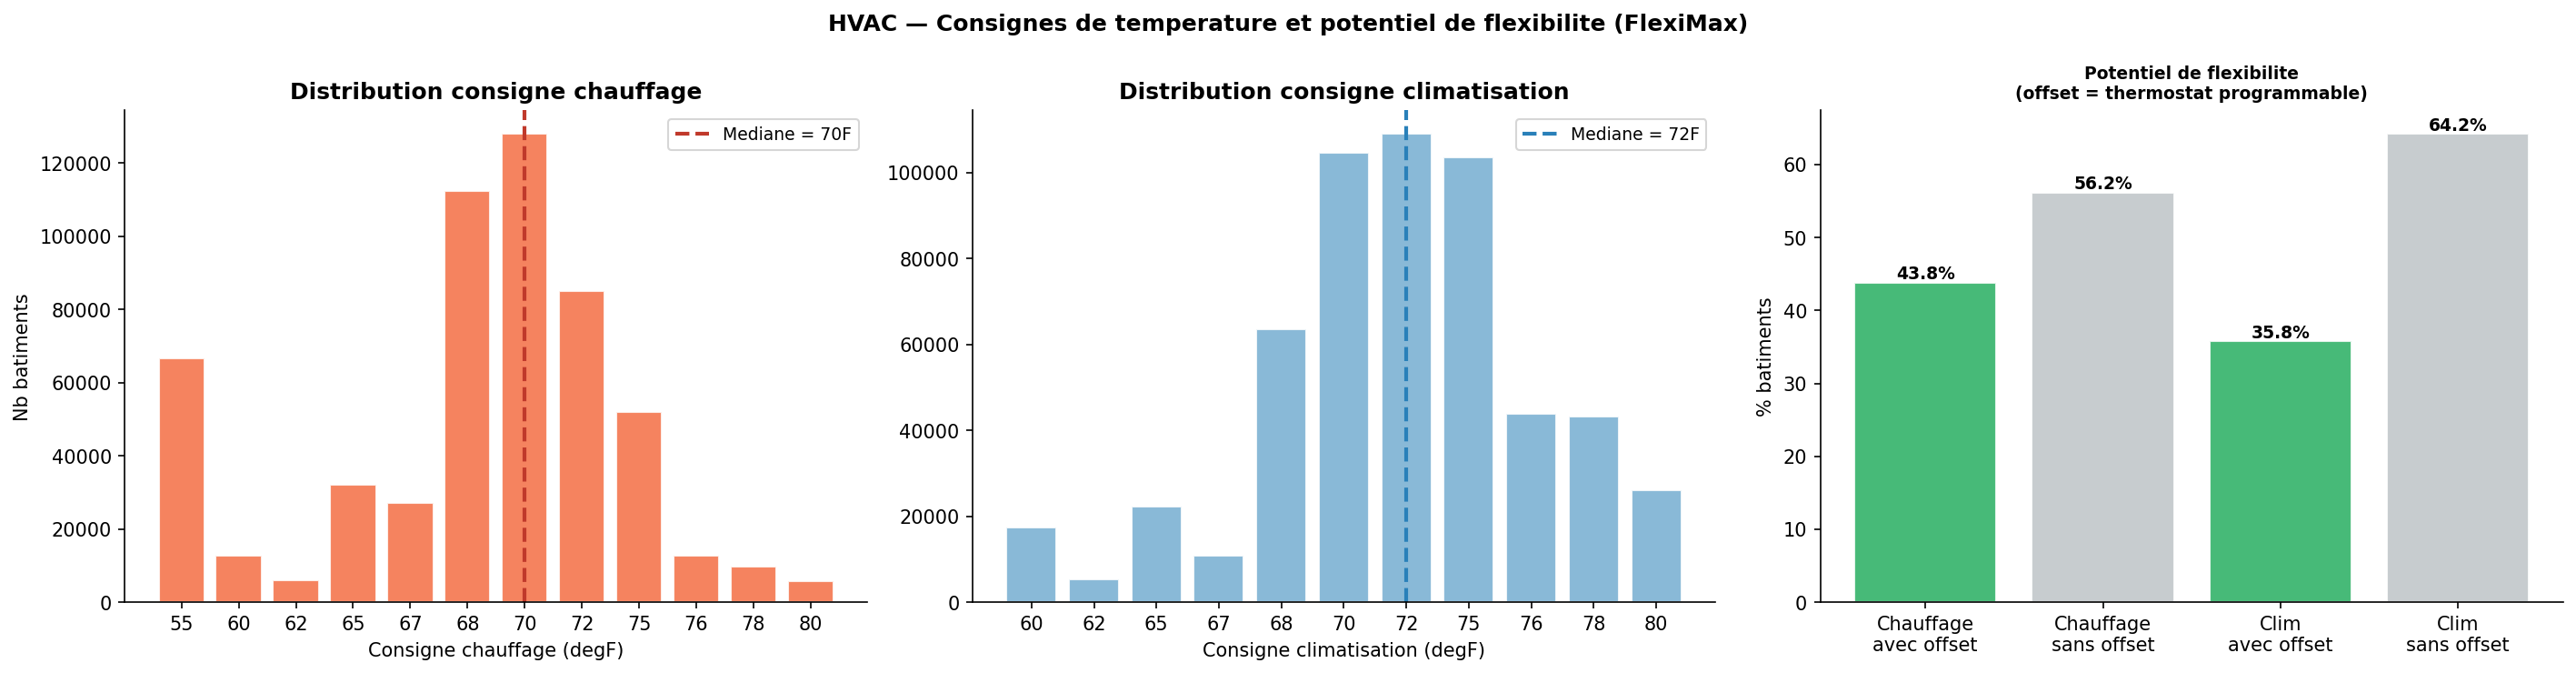
\includegraphics[width=0.82\textwidth]{hvac_setpoints_flexibilite.png}
  \caption{Consignes de température et potentiel de flexibilité (part des bâtiments avec
  thermostat programmable).}
  \label{fig:hvac-setpoints}
\end{figure}

\begin{figure}[htbp]
  \centering
  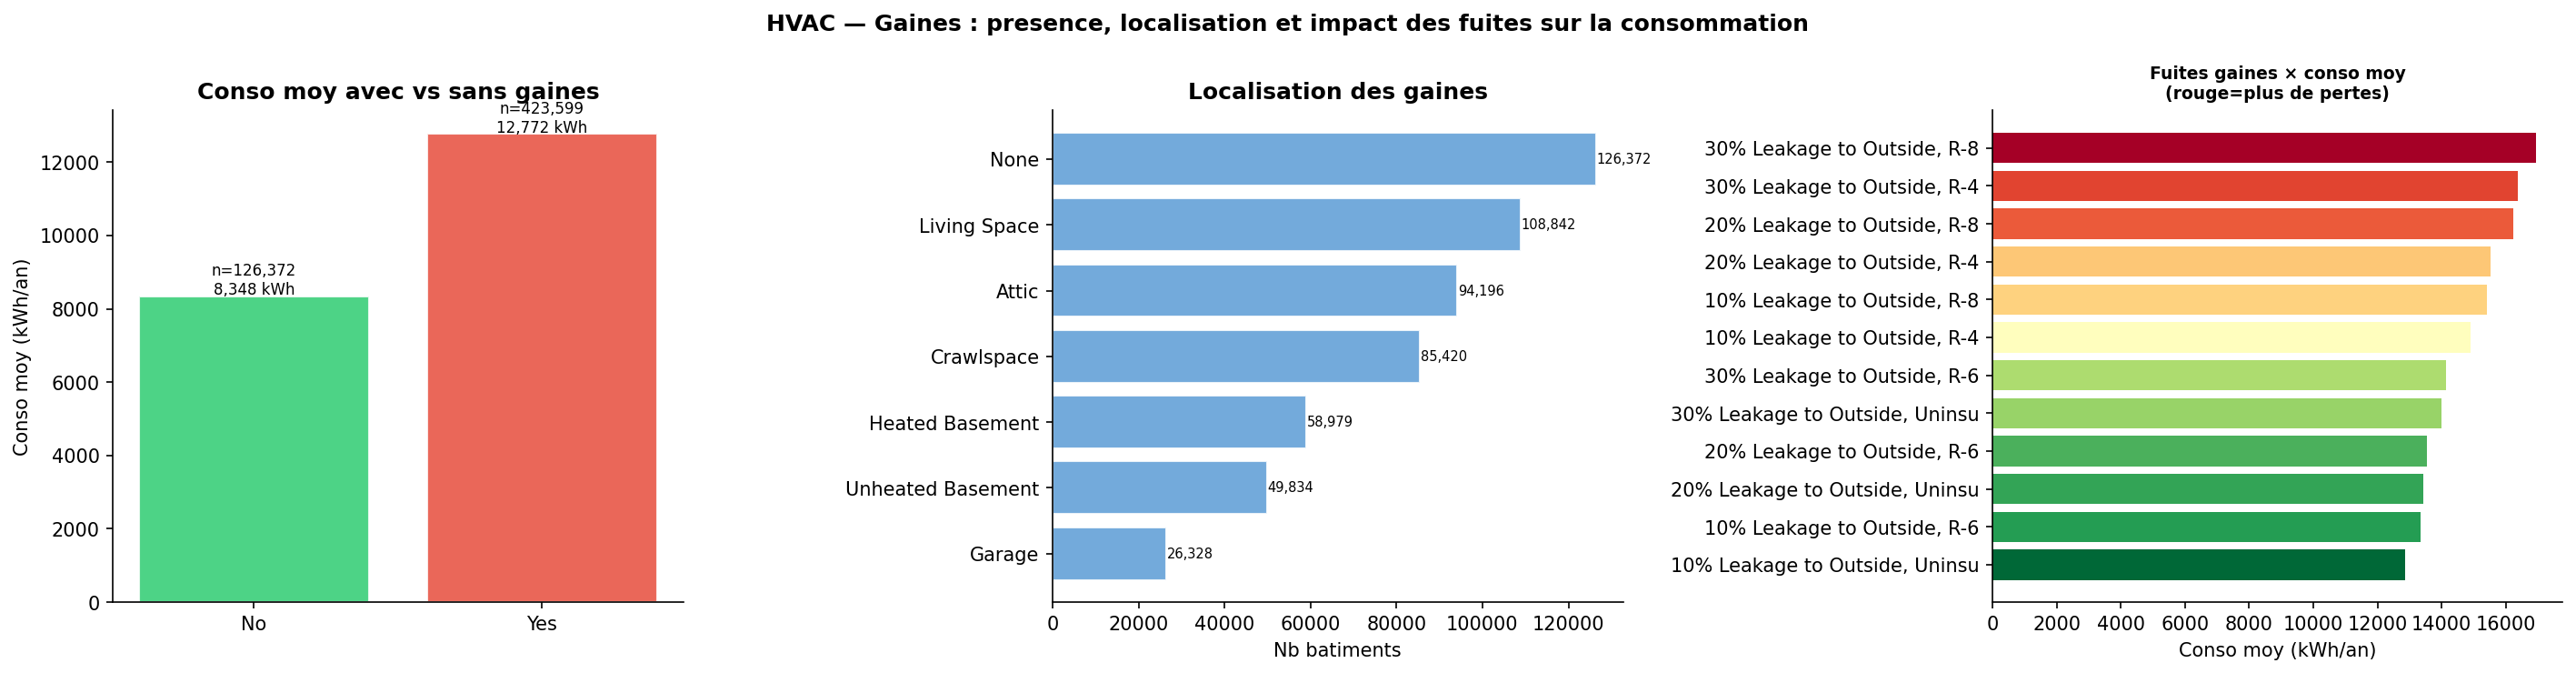
\includegraphics[width=0.82\textwidth]{hvac_gaines.png}
  \caption{Présence et localisation des gaines de distribution d'air ; impact des fuites sur la
  consommation.}
  \label{fig:hvac-gaines}
\end{figure}

\section{Occupants et profil socio-économique}
\begin{resultbox}[Source : \code{exploration\_occupants.ipynb}]
Sur le \emph{vintage} du bâti, un paradoxe apparent : plus un bâtiment est récent, plus sa
consommation \emph{absolue} est élevée (10\,013~kWh/an avant 1940 à 12\,659~kWh/an années 2000),
alors que l'\emph{intensité} (kWh/ft²) est minimale pour les années 2010 (7,0~kWh/ft²) - les
constructions récentes sont plus efficaces par m², mais en moyenne plus grandes. Côté occupants,
la relation est quasi linéaire avec la consommation moyenne : de $\sim$4\,100~kWh/an à 0
occupant (vacant) à $\sim$21\,700~kWh/an à 9 occupants. Les foyers de 2 personnes dominent
(167\,006 bâtiments), suivis des foyers d'une personne (132\,575).
\end{resultbox}

\begin{figure}[htbp]
  \centering
  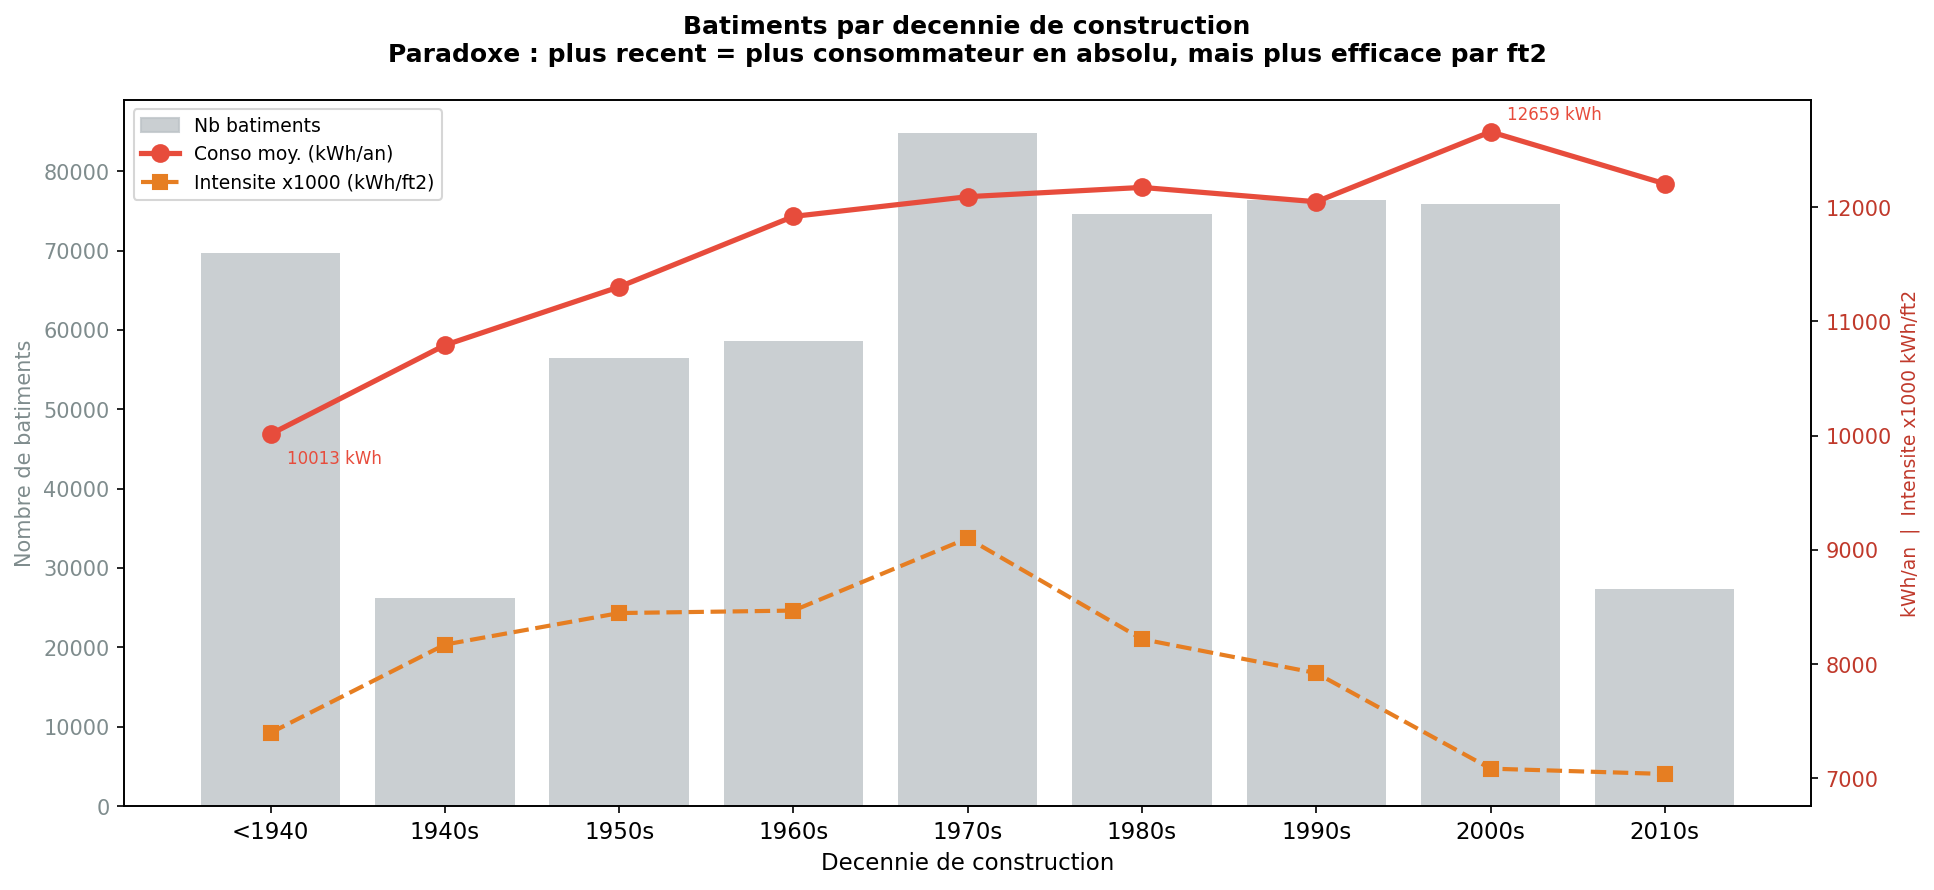
\includegraphics[width=0.75\textwidth]{vintage_timeline.png}
  \caption{Consommation moyenne et intensité (kWh/ft²) par décennie de construction.}
  \label{fig:vintage-timeline}
\end{figure}

\begin{figure}[htbp]
  \centering
  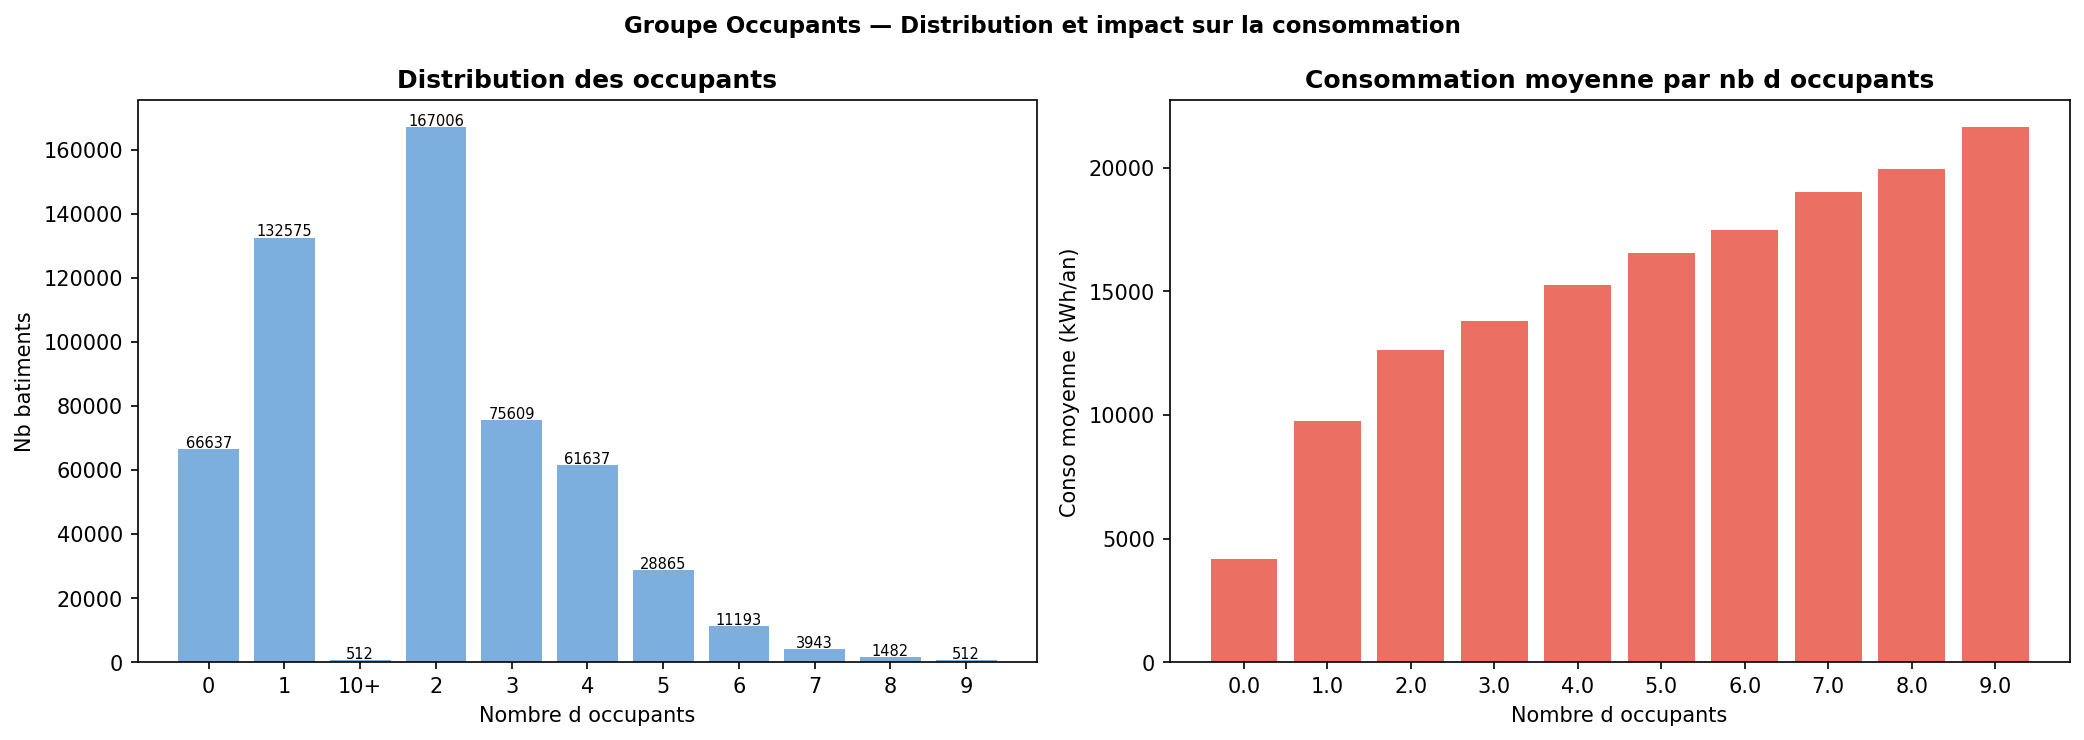
\includegraphics[width=0.78\textwidth]{occupants_distribution.png}
  \caption{Distribution du nombre d'occupants et consommation moyenne associée.}
  \label{fig:occupants-distrib}
\end{figure}

\section{Classification métier des variables}
\label{sec:classification-metier}
Enveloppe, HVAC, occupants : ces familles explorées séparément gagnent à être mises en regard des
usages électriques eux-mêmes, pour juger lesquelles sont réellement pilotables.
\begin{resultbox}[Source : \code{03\_visualisation/classification\_variables.ipynb}]
Ce notebook croise les 165 variables \code{in.*} avec les usages électriques
\code{out.electricity.*} pour produire une classification « métier » (plutôt que technique),
utilisée comme grille de lecture pour la suite du rapport :
\begin{itemize}
  \item \textbf{61} variables retenues (Enveloppe 33\%, HVAC 16\%, Socio-économique 11\%,
  Météo/climat 10\%, Comportemental 9\%, Eau chaude 6\%, Occupants/VE/PV 5\% chacun),
  \textbf{16} écartées (redondantes ou non pilotables) ;
  \item Décomposition de la \emph{consommation électrique} moyenne (11\,756~kWh/an, tous usages
  électriques confondus) : climatisation (27,4\%), électronique « brun » (20,6\%), chauffage
  (19,3\%), électroménager « blanc » (14,5\%), eau chaude (8,2\%), éclairage (7,5\%), divers
  (1,9\%) - climatisation et chauffage électriques combinés (46,7\% \emph{de l'électricité})
  restent le premier poste, mais l'écart avec l'« électronique brun » (non pilotable, 20,6\%)
  borne le gain maximal atteignable par la seule flexibilité thermique. \emph{À ne pas confondre
  avec la part du confort thermique tous vecteurs confondus (64,2\%, \S\ref{sec:visual-national})
  : cette dernière inclut aussi le chauffage au gaz, propane et fioul, absent ici.} ;
  \item Cas \code{in.neighbors} : pas un proxy météo mais une variable de mitoyenneté (67,7\%
  de maisons individuelles), gardée comme feature d'enveloppe plutôt qu'écartée comme
  redondante ;
  \item VE : 1,1\% des ménages seulement, mais consommation de recharge moyenne de
  2\,082~kWh/an (contre 22~kWh/an sur l'ensemble du parc) - marginal en pénétration mais
  fortement pilotable, à traiter séparément de l'analyse thermique.
\end{itemize}
Cette classification par catégorie, plutôt qu'une liste plate de 61 variables, servira de grille
de lecture pour l'importance des variables du futur modèle prédictif : elle permettra de juger
si un déterminant dominant relève du bâti, du climat ou du comportement, plutôt que d'interpréter
chaque variable isolément.
\end{resultbox}

\begin{figure}[htbp]
  \centering
  \includegraphics[width=\textwidth]{classification_usages_et_categories.png}
  \caption{Décomposition de la consommation électrique moyenne par usage (chauffage,
  climatisation, eau chaude, électroménager « blanc », électronique « brun »...) et répartition
  des variables retenues par catégorie métier.}
  \label{fig:classif-usages}
\end{figure}

\begin{resultbox}[Schéma hiérarchique - consommation électrique et facteurs explicatifs]
\begin{footnotesize}
\begin{alltt}
CONSOMMATION ELECTRIQUE RESIDENTIELLE
|
+-- Chauffage          -> out.electricity.heating.*          Pilotable (thermostat)
+-- Climatisation      -> out.electricity.cooling.*           Pilotable (setpoint offset)
+-- Eau chaude (DHW)   -> out.electricity.hot_water.*          Pilotable (heure de chauffe)
+-- Eclairage          -> out.electricity.lighting_* + ceiling_fan   Pilotable partiel
+-- Ventilation        -> out.electricity.mech_vent            Pilotable partiel
+-- Usages specifiques
|     +-- Blanc (electromenager) : lave-linge, seche-linge, lave-vaisselle,
|     |     refrigerateur, congelateur, cuisiniere       Pilotable partiel (horaires decalables)
|     +-- Brun (electronique) : television, plug_loads          Non pilotable
+-- VE (traitement separe) -> ev_charging               Pilotable (recharge decalable)

FACTEURS EXPLICATIFS
+-- Occupants          in.occupants, in.usage_level, in.vacancy_status
+-- Comportement        in.heating_setpoint*, in.cooling_setpoint*, in.*_usage_level
+-- Meteo (proxys)      in.ashrae_iecc_climate_zone_2004, in.weather_file_latitude/longitude
+-- Enveloppe thermique in.insulation_*, in.air_leakage_*, in.windows, in.geometry_*, in.neighbors
+-- HVAC                in.hvac_heating_type, in.hvac_cooling_type, in.hvac_*_efficiency
+-- Socio-economique    in.income, in.federal_poverty_level, in.tenure, in.area_median_income
\end{alltt}
\end{footnotesize}
\end{resultbox}

\section{Décomposition nationale par usage et par vecteur énergétique}
\label{sec:visual-national}
La classification précédente porte sur l'électricité seule. Élargie à \emph{tous} les vecteurs
énergétiques (gaz, propane, fioul inclus), la même décomposition par usage change-t-elle
d'équilibre ?
\begin{resultbox}[Source : \code{03\_visualisation/visual.ipynb} - \code{upgrade0.parquet} - ménages pondérés]
Sur le parc entier (549\,971 bâtiments pondérés), le confort thermique (chauffage + climatisation,
\emph{tous vecteurs}) concentre \textbf{64,2\%} de la consommation totale, loin devant l'eau chaude
sanitaire (12,0\%) et le divertissement/loisirs (11,3\%). Ce chiffre est plus élevé que les 46,7\%
mesurés pour l'électricité seule (\S\ref{sec:classification-metier}) : l'écart est le gaz, le
propane et le fioul consacrés au chauffage, invisibles dans une lecture électricité-only. Par
vecteur, l'électricité (1\,641,5~TWh) et le gaz naturel (1\,479,1~TWh) sont proches en volume
national, très loin devant le fioul (178,8~TWh) et le propane (154,1~TWh). La décomposition par
groupe montre où se concentre ce gaz : quasi exclusivement sur le confort thermique et, dans une
moindre mesure, l'eau chaude sanitaire et l'alimentation - tous les autres usages
(divertissement, éclairage, VE, infrastructure, PV) sont déjà quasi 100\% électriques. Cette
proximité électricité/gaz, concentrée sur les usages thermiques, confirme à l'échelle nationale
l'intérêt du recentrage tout-électrique du périmètre.
\end{resultbox}

\begin{figure}[htbp]
  \centering
  \begin{subfigure}[b]{0.48\textwidth}
    \centering
    
\includegraphics[width=\textwidth]{viz2_camembert_groupes.png}
    \caption{Par usage fonctionnel.}
    \label{fig:viz-camembert}
  \end{subfigure}
  \hfill
  \begin{subfigure}[b]{0.48\textwidth}
    \centering
    
\includegraphics[width=\textwidth]{viz4_barres_empilees.png}
    \caption{Par groupe et par vecteur énergétique.}
    \label{fig:viz-energie}
  \end{subfigure}
  \caption{Répartition de la consommation nationale totale (tous vecteurs, ménages pondérés).}
  \label{fig:viz-repartition-nationale}
\end{figure}

\begin{resultbox}[Corrélations entre usages - \code{03\_visualisation/visual.ipynb}]
Deux logiques se distinguent. Un \textbf{cluster « comportemental »} (eau chaude sanitaire,
hygiène/nettoyage, divertissement) est fortement corrélé en interne ($\rho=0,50$ à $0,62$) : ces
usages suivent l'intensité d'occupation du logement. Le \textbf{confort thermique}, pourtant
premier poste (64,2\%), n'est que faiblement corrélé aux autres ($\rho=0,21$ à $0,35$) - sa
variance dépend du bâti et du climat, pas du comportement, cohérent avec le rôle de la zone
climatique comme déterminant n°1 (\S\ref{sec:localisation-climat}). VE et PV sont quasi
indépendants de tout le reste ($|\rho|<0,05$) : des choix d'équipement, pas de comportement.
\emph{Utilité :} un seul proxy d'occupation suffira à résumer le cluster comportemental en
feature engineering (\S\ref{sec:principe-encodage}), alors que confort thermique, VE et PV
garderont chacun leurs propres variables et leviers de flexibilité dédiés.
\end{resultbox}

\begin{figure}[htbp]
  \centering
  \includegraphics[width=0.75\textwidth]{viz6_heatmap_correlation.png}
  \caption{Corrélation de Pearson entre les consommations par groupe fonctionnel.}
  \label{fig:viz-correlation}
\end{figure}

% ============================================================================
\chapter{De la donnée brute à la feature physique}
\label{ch:features}

Ce chapitre transforme les variables \code{in.*} encodées jusqu'ici en catégories ResStock en un
jeu de features numériques, à partir des notebooks \code{transformations\_numeriques.ipynb} et
\code{encodage\_categoriel.ipynb}.

\section{Principe d'encodage}
\label{sec:principe-encodage}
\begin{resultbox}[Source : \code{transformations\_numeriques.ipynb} + \code{encodage\_categoriel.ipynb}]
Chaque variable \code{in.*} est encodée selon sa nature : valeur numérique conservée telle
quelle, table de correspondance officielle du \emph{ResStock Technical Reference Guide} (isolation,
vitrage), extraction de la valeur numérique dans une chaîne composite (ex. cote SEER, EF, IMEF,
CEF), encodage binaire ou one-hot pour les catégories nominales sans ordre, et encodage circulaire
(sinus/cosinus) pour l'orientation, une variable cyclique (0°=360°) qu'un simple entier
briserait artificiellement en deux extrêmes opposés.

Cas notable : l'isolation est encodée par sa \textbf{valeur R d'assemblage} (celle réellement
utilisée par EnergyPlus, incluant les ponts thermiques de l'ossature, Table~45 du guide) plutôt
que sa valeur R \textbf{nominale} (celle affichée sur le produit) - l'écart croît avec la
conductivité de la structure porteuse : un mur à ossature bois isolé R-11 (nominal) descend à
10,3 en valeur d'assemblage, R-15 à 12,1. Un encodage sur la seule valeur nominale surestimerait
donc la performance thermique réelle des parois.

Sept variables sont supprimées car constantes sur tout le parc (\code{in.interior\_shading},
\code{overhangs}, \code{eaves}, \code{doors}, \code{radiant\_barrier}, \code{infiltration},
\code{door\_area}) : une variance nulle ne porte aucune information exploitable, quel que soit
l'encodage choisi.

\begin{table}[H]
\centering
\caption{Les 108 attributs \code{in.*} encodés dans \code{X.parquet}, par groupe métier.}
\label{tab:encodage-groupes}
\begin{tabular}{@{}p{4.4cm}r p{8.9cm}@{}}
\toprule
Groupe & Var. & Encodage principal appliqué \\
\midrule
1 Socio-économique         & 7  & Midpoint d'intervalle (\$), ratio, binaire \\
2 Occupants                 & 6  & Numérique, binaire, label ordinal \\
3 Météo                      & 2  & Numérique (latitude/longitude, inchangé) \\
4 Enveloppe thermique        & 32 & Lookup R d'assemblage, OHE finitions, circulaire orientation \\
5 Systèmes HVAC/DHW          & 25 & Conversion \degree F$\to$\degree C, extraction SEER/EF, OHE techno./combustible \\
6 Usages électriques         & 25 & Extraction CEF/EF, binaire présence, OHE énergie \\
7 Blanc/Brun                  & 4  & Ratio (\%$\to$décimal), numérique \\
8 Infrastructure électrique   & 2  & Numérique (A, count - inchangé) \\
9 Photovoltaïque (PV)         & 2  & Binaire, extraction puissance (kW) \\
10 Mobilité (VE)               & 3  & Numérique, label niveau de chargeur \\
\midrule
\textbf{Total} & \textbf{108} & \\
\bottomrule
\end{tabular}
\end{table}
Le groupe Enveloppe (32 variables, 30\% du total) domine largement : c'est ce volume, et sa
spécificité au parc états-unien (catégories ResStock plutôt que grandeurs physiques directes),
qui motive l'agrégation du \S\ref{sec:agregation-physique}.
\end{resultbox}

\section{Agrégation physique de l'enveloppe}
\label{sec:agregation-physique}
\begin{resultbox}[Source : \code{05\_deeplearning/lgbm\_electricity\_5features.ipynb} - sous-ensemble tout-électrique plain-pied - 64\,062 logements]
Pour une variante physiquement interprétable du modèle prédictif (\code{05\_deeplearning}), un
sous-ensemble filtré (maisons individuelles à un niveau, chauffage électrique, sans VE ni piscine
ni PV - une restriction plus étroite que le recentrage tout-électrique du rapport) recalcule,
à partir des colonnes \code{out.params.*} et des variables encodées au \S\ref{sec:principe-encodage},
30 attributs bruts d'enveloppe en \textbf{5 grandeurs physiques universelles} :
\begin{table}[H]
\centering
\caption{Les 5 agrégats physiques (modèle RC) remplaçant 30 attributs bruts d'enveloppe.}
\label{tab:agregats-physiques}
\begin{tabular}{lp{5.6cm}p{5.4cm}}
\toprule
Agrégat & Formule (résumée) & Rôle physique \\
\midrule
$UA$ (W/K) & $\sum_i U(R_i)A_i + U_\mathrm{fen}A_\mathrm{fen} + 1{,}14\,A_\mathrm{porte}$ &
Pertes par transmission (murs, toit, plancher, fenêtres, portes) \\
$H_{ve}$ (W/K) & $0{,}34\,(\mathrm{ACH50}/20)\,V$ &
Pertes par renouvellement d'air / infiltration \\
$C$ (kJ/K) & $C_\mathrm{classe}\times A_\mathrm{pl}$, classes ISO~13790 $\in\{110,165,260,370\}$ &
Inertie thermique, selon matériau structurel \\
$A_\mathrm{solaire}$ (m$^2$) & $\mathrm{SHGC}\times 0{,}9\times\sum A_\mathrm{fen}\times
p(\theta)$, Sud$>$Est/Ouest$>$Nord & Gains solaires équivalents \\
compacité (m$^{-1}$) & $(A_\mathrm{mur}\!+\!A_\mathrm{toit}\!+\!A_\mathrm{pl}\!+\!A_\mathrm{fen}\!+
\!A_\mathrm{porte})/V$ & Coefficient de forme (compacité du bâti) \\
\bottomrule
\end{tabular}
\end{table}

\textbf{Bilan :} 108 attributs bruts $\to$ 83 features (5 agrégats physiques + 78 conservés tels
quels). Seul le bloc enveloppe (30 attributs) est fondu dans les agrégats ; le reste - HVAC,
gaines, eau chaude, occupants, socio-économique, usages électriques - est conservé sans
élagage supplémentaire à ce stade. Réduire une trentaine de catégories propres au parc
états-unien à cinq grandeurs physiques sert un double objectif : la \textbf{transférabilité} -
ces grandeurs ont un sens hors ResStock, sur un parc de logements différent - et
l'\textbf{interprétabilité}, en vue d'un modèle thermique de type RC (résistance-capacité)
plutôt qu'une boîte noire sur 108 colonnes hétérogènes. L'importance de ces agrégats dans le
modèle prédictif est vérifiée au chapitre~\ref{ch:modelisation}.
\end{resultbox}

Le détail complet des 108 attributs - variable par variable, avec statut réel (conservé, supprimé ou fondu dans un agrégat) - est reporté en annexe~\ref{app:variables-detail} pour ne pas alourdir ce chapitre.

% ============================================================================
\chapter{Modélisation}
\label{ch:modelisation}

Le climat structure la consommation (chapitre~\ref{ch:exploration}), l'enveloppe et les
équipements expliquent une partie de la dispersion résiduelle (chapitre~\ref{ch:beyond-climate}),
et 108 attributs bruts ont été réduits à un jeu de features exploitable, physique ou complet
(chapitre~\ref{ch:features}). Ce chapitre vérifie si un modèle prédictif retrouve effectivement
ces déterminants, et jusqu'à quel point il peut prédire la consommation électrique.

\section{Un modèle LightGBM sur le périmètre tout-électrique}
\label{sec:lgbm-electricite}
\begin{resultbox}[Source : \code{05\_deeplearning/lgbm\_electricity.ipynb} - sous-ensemble tout-électrique plain-pied - 64\,062 logements]
Un LightGBM entraîné sur les 107 features encodées (\S\ref{sec:principe-encodage}), avec split
stratifié par zone ASHRAE (Train 40\,999 / Val 10\,250 / Test 12\,813) et 50 essais
d'optimisation Optuna, atteint sur le test $R^2=0{,}9254$ (RMSE $=2\,712$~kWh, soit 13,8\% de la
consommation moyenne ; écart train/test $=0{,}057$, contrôlé). C'est une nette amélioration par
rapport au premier modèle du stage, entraîné avant le recentrage tout-électrique sur les
549\,971 bâtiments et les cinq vecteurs énergétiques (\code{lightgbm\_stratified.ipynb},
$R^2=0{,}8446$, RMSE $=28{,}9\%$) : le gain ($+0{,}08$ de $R^2$, RMSE relative divisée par deux)
tient moins à un modèle différent qu'au périmètre lui-même - un sous-ensemble tout-électrique
et géométriquement homogène, sur une cible unique, stratifié directement sur la zone climatique
plutôt que sur une stratification composite plus généraliste.
\end{resultbox}

\begin{figure}[htbp]
  \centering
  \includegraphics[width=0.85\textwidth]{modelisation_comparaison_electricite.png}
  \caption{$R^2$, RMSE et RMSE relative  -  modèle multi-cibles pré-recentrage
  (\code{lightgbm\_stratified}) vs modèle électricité sur le périmètre tout-électrique
  (\code{lgbm\_electricity}).}
  \label{fig:modelisation-comparaison}
\end{figure}

L'erreur par zone climatique (test) confirme le fil conducteur du rapport : les zones rares et
extrêmes (7B, $n=8$, RMSE $=9\,044$~kWh ; 6A, $n=233$, RMSE $=4\,168$~kWh) concentrent l'essentiel
de l'erreur et du biais, tandis que les zones tempérées majoritaires (2A, 3A, 4A) restent sous
3\,300~kWh de RMSE, une limite de taille d'échantillon plus qu'une faiblesse du modèle.

\section{Global vs Physique : le compromis interprétabilité}
\label{sec:global-vs-physique}
\begin{resultbox}[Source : \code{05\_deeplearning/lgbm\_electricity\_5features.ipynb} - même sous-ensemble - 64\,062 logements]
Remplacer les 30 attributs bruts d'enveloppe par les 5 agrégats physiques du
\S\ref{sec:agregation-physique} (83 features au lieu de 107, jeu \og Physique\fg) coûte peu :
$R^2=0{,}9120$ (RMSE $=2\,945$~kWh, 15,0\%) contre $0{,}9254$ pour le jeu \og Global\fg{} - une
perte de 1,3 point de $R^2$ pour cinq variables interprétables en moins de description physique
du bâti. L'importance des variables confirme que cette perte est mesurée, pas accidentelle : $UA$
arrive en 2\textsuperscript{e} position (8,85\% de l'importance totale, juste derrière la latitude
météo), et les 5 agrégats cumulés pèsent \textbf{32,3\%} de l'importance du modèle - l'enveloppe
compte, même réduite à cinq nombres. La latitude et la longitude météo dominent toujours
largement (18,4\% cumulés), confirmant à l'échelle du modèle prédictif ce que l'exploration
suggérait déjà (\S\ref{sec:localisation-climat}) : le climat prime sur le bâti. Une courbe du
coude sur le nombre de features retenues montre par ailleurs que la moitié des attributs
(50 sur 83, ou 80 sur 107 pour le jeu Global) suffit à retrouver la performance du jeu complet - 
la longue traîne de variables à faible importance (VE, PV, spa, piscine, redondantes avec le
filtre du sous-ensemble) n'apporte rien de plus.
\end{resultbox}

\section{Performance par usage électrique}
\label{sec:performance-usages}
\begin{resultbox}[Source : \code{05\_deeplearning/lgbm\_electricity\_5features.ipynb} - quatre modèles - mêmes features et split]
Prédire chaque usage séparément (mêmes 83 features, mêmes hyperparamètres qu'en
\S\ref{sec:global-vs-physique}) révèle une hétérogénéité nette : l'eau chaude sanitaire est
l'usage le plus facile ($R^2=0{,}980$, RMSE $=214$~kWh) et le chauffage le plus difficile
($R^2=0{,}816$, RMSE relative $=54{,}0\%$). Ce n'est pas un défaut du modèle mais une conséquence
de la variance du signal : la consommation de chauffage varie fortement d'un ménage à l'autre
(moyenne 6\,030~kWh, mais 98,9\% des logements seulement en ont - contre 84,6\% pour l'eau
chaude, dont la consommation moyenne, plus faible et plus stable, est mécaniquement plus facile à
approcher en valeur relative). La climatisation se situe entre les deux ($R^2=0{,}930$,
18,9\%). Ce classement, eau chaude $>$ climatisation $>$ total $>$ chauffage, est cohérent
avec le rôle du climat déjà établi : le chauffage est l'usage le plus exposé à la variabilité
climatique inter-zones, donc le plus dur à généraliser sur un modèle unique.
\end{resultbox}

\begin{figure}[htbp]
  \centering
  \includegraphics[width=0.85\textwidth]{modelisation_par_usage.png}
  \caption{$R^2$ et RMSE par usage électrique (total, chauffage, climatisation, eau chaude),
  jeu de features Physique.}
  \label{fig:modelisation-par-usage}
\end{figure}

\begin{figure}[htbp]
  \centering
  \includegraphics[width=0.85\textwidth]{modelisation_importance_agregats.png}
  \caption{Importance des 83 variables du jeu Physique (gain LightGBM)  -  les 5 agrégats
  physiques en rouge.}
  \label{fig:modelisation-importance}
\end{figure}

% ============================================================================
\chapter{Dynamique temporelle}
\label{ch:dynamique-temporelle}

Les chapitres précédents traitent la consommation électrique comme une grandeur annuelle : un
seul nombre par logement, expliqué par le climat, le bâti et les équipements
(chapitres~\ref{ch:exploration} à \ref{ch:modelisation}). Or l'électricité qui compte pour la
flexibilité se joue à l'heure, pas à l'année. Ce chapitre explore la dimension temporelle sur le
même périmètre tout-électrique~: d'abord en cherchant des \og jours types \fg{} par clustering non
supervisé des profils journaliers, à l'échelle d'un bâtiment puis d'un panel de 100 bâtiments,
puis en entraînant un modèle hybride RNN+MLP pour prédire la consommation à deux horizons
(l'heure suivante, et le total annuel à partir de 90 jours observés).

\section{Jours types~: clustering du profil journalier d'un bâtiment de référence}
\label{sec:clustering-jours-types}
Avant tout traitement, les profils journaliers bruts d'un bâtiment sur une année entière
(figure~\ref{fig:clustering-jours-types-brut}) ne montrent aucune structure évidente à l'œil
nu~: c'est précisément ce que le clustering non supervisé qui suit cherche à organiser en
régimes identifiables.

\begin{figure}[htbp]
  \centering
  \includegraphics[width=0.85\textwidth]{timeseries_clustering_exemple_profil_horaire.png}
  \caption{Les 365 profils horaires bruts d'un bâtiment (347201-0, exemple illustratif),
  superposés (semaine en bleu, weekend en rouge) - avant toute normalisation ou clustering. Le
  bâtiment de référence pour l'analyse qui suit (10672-0) est introduit ci-dessous.}
  \label{fig:clustering-jours-types-brut}
\end{figure}

\begin{resultbox}[Source : \code{06\_timeseries/timeseries\_clustering.ipynb} - bâtiment 10672-0 - pas 15 minutes]
Chaque journée (pas 15~minutes, 96 valeurs $x_1,\dots,x_{96}$) est normalisée de deux façons
concurrentes, qui ne portent pas sur le même axe de la matrice jours$\times$pas de temps.

\textbf{Forme} - z-score \emph{intra-jour} (par \emph{ligne})~: pour un jour $j$ donné,
$x_{j,i}^{\text{forme}} = (x_{j,i} - \bar{x}_j) / \sigma_j$, où $\bar{x}_j$ et $\sigma_j$ sont la
moyenne et l'écart-type calculés sur les 96 valeurs de \emph{ce jour} uniquement. Chaque jour est
donc recentré-réduit sur sa propre échelle~: le niveau absolu disparaît complètement, seule
reste la position relative des pics et des creux dans la journée.

\textbf{Amplitude} - \code{StandardScaler} \emph{global} (par \emph{colonne})~: pour un pas de
temps $i$ (une heure de la journée) donné, $x_{j,i}^{\text{amplitude}} = (x_{j,i} - \bar{x}_i) /
\sigma_i$, où $\bar{x}_i$ et $\sigma_i$ sont cette fois calculés sur \emph{ce même pas de temps},
à travers \emph{tous} les jours de l'année. La consommation de 8h un jour donné est donc comparée
à la consommation moyenne à 8h sur l'année entière~: les écarts de niveau global entre un jour
creux et un jour très consommateur sont \emph{préservés}, contrairement à la forme.

Un K-Means est ajusté séparément sur chaque représentation, avec $k$
choisi par méthode du coude puis vérifié par score de silhouette. Les deux normalisations
retiennent toutes deux $k=5$, mais avec des profils de silhouette très différents~: la forme
culmine à $k=3$ (0,29) puis décroît (0,21 à $k=5$) - des tailles de cluster 46/79/129/71/40,
avec un recouvrement net entre formes voisines ; l'amplitude culmine dès $k=2$ (0,56) et reste
élevée à $k=5$ (0,39, tailles 24/231/11/70/29) - un clustering nettement mieux séparé, porté par
un cluster majoritaire (231 jours, le régime courant) entouré de clusters minoritaires qui captent
les jours extrêmes.
\end{resultbox}

\begin{figure}[htbp]
  \centering
  \begin{subfigure}[b]{0.48\textwidth}
    \centering
    \includegraphics[width=\textwidth]{timeseries_clustering_coude_10672_forme.png}
    \caption{Forme  -  $k=5$ retenu, silhouette maximale 0,29 (à $k=3$).}
  \end{subfigure}
  \hfill
  \begin{subfigure}[b]{0.48\textwidth}
    \centering
    \includegraphics[width=\textwidth]{timeseries_clustering_coude_10672_amplitude.png}
    \caption{Amplitude  -  $k=5$ retenu, silhouette maximale 0,56 (à $k=2$).}
  \end{subfigure}
  \caption{Méthode du coude et score de silhouette pour les deux normalisations  -  bâtiment
  10672-0.}
  \label{fig:clustering-jours-types-coude}
\end{figure}

La figure~\ref{fig:clustering-jours-types-coude} rend visible l'écart entre les deux
normalisations~: le score de silhouette de l'amplitude reste au-dessus de 0,29 sur toute la plage
$k=2$ à $k=9$, contre un plafond à 0,29 (atteint une seule fois, à $k=3$) puis une chute continue
pour la forme - un clustering objectivement plus net, cohérent avec le diagnostic du texte
ci-dessus.

\begin{figure}[htbp]
  \centering
  \begin{subfigure}[b]{\textwidth}
    \centering
    \includegraphics[width=0.85\textwidth]{timeseries_clustering_profils_10672_forme.png}
    \caption{Forme  -  profils normalisés par cluster (moyenne $\pm$ écart-type).}
  \end{subfigure}
  \begin{subfigure}[b]{\textwidth}
    \centering
    \includegraphics[width=0.85\textwidth]{timeseries_clustering_profils_10672_amplitude.png}
    \caption{Amplitude  -  profils en kWh par cluster (moyenne $\pm$ écart-type).}
  \end{subfigure}
  \caption{Courbes de consommation moyenne par cluster, sur 24h  -  bâtiment 10672-0.}
  \label{fig:clustering-jours-types-profils}
\end{figure}

Les courbes de la figure~\ref{fig:clustering-jours-types-profils} donnent un visage concret aux
clusters~: pour l'amplitude, le cluster majoritaire (1, $n=231$) reste plat et bas toute la
journée, tandis que les clusters minoritaires (0, 2, 3, 4) affichent des niveaux et des pics
(vers 12h et 22h) nettement plus marqués - une différence de \emph{palier}, pas de forme.
Pour la forme, les 5 courbes se chevauchent visiblement sur la journée, avec des pics communs à
11-12h et 21-22h dont seule l'amplitude relative diffère, ce chevauchement visuel est la
contrepartie directe de la silhouette faible mesurée plus haut.

La composition calendaire des clusters de forme confirme un résultat plus riche qu'une simple
opposition saison/semaine~: les clusters 1 ($n=79$) et 4 ($n=40$) sont tous deux concentrés en
hiver (novembre--février), mais s'opposent presque parfaitement sur le rythme hebdomadaire - 
100\% de jours de semaine pour le cluster 1, 77,5\% de weekend pour le cluster 4. À l'inverse, les
clusters 0 ($n=46$) et 2 ($n=129$) se recoupent sur la saison estivale (mai--septembre) sans
opposition semaine/weekend marquée. Le climat (chapitre~\ref{ch:exploration}) structure donc bien
la forme du profil journalier, mais le rythme hebdomadaire s'y superpose - les deux facteurs
n'agissent pas au même niveau, la saison fixant le \emph{régime} et la semaine modulant son
\emph{occurrence}.

\begin{resultbox}[Source : \code{06\_timeseries/timeseries\_clustering.ipynb} - décomposition par poste - bâtiment 10672-0]
Les métadonnées statiques du foyer (revenu 15\,000--19\,999\$, sous le seuil de pauvreté fédéral ;
3 occupants ; locataire ; bâtiment des années 1950 ; chauffage gainé, climatisation centrale) ne
disent rien de \emph{quand} la consommation varie dans la journée, elles ne portent aucune
information temporelle. La décomposition par poste, elle, est directe~: le \textbf{chauffage}
domine presque entièrement chaque courbe et porte, à lui seul, les deux pics à 11--12h et 21--22h
sur les clusters d'hiver (0, 2, 3, 4 en amplitude) - les autres postes (eau chaude, réfrigérateur,
éclairage) restent une fine bande quasi plate en comparaison. Le cluster majoritaire (amplitude,
$n=231$) est quasiment plat toute la journée précisément parce que le chauffage y est
quasi nul, des journées assez douces pour ne pas en avoir besoin. Ce motif à deux pics
quotidiens est cohérent avec la métadonnée \code{in.heating\_setpoint\_has\_offset = Yes}~: ce
foyer dispose d'un thermostat programmable pour le chauffage, et le double pic correspond au cycle
classique d'abaissement/relance (nuit puis journée d'absence, relance le matin et en début de
soirée) plutôt qu'à un usage continu.
\end{resultbox}

\begin{figure}[htbp]
  \centering
  \includegraphics[width=0.95\textwidth]{timeseries_clustering_par_poste_10672_amplitude.png}
  \caption{Décomposition par poste de consommation, profils d'amplitude par cluster  -  bâtiment
  10672-0. Le chauffage (hachures vertes) domine et porte les pics.}
  \label{fig:clustering-jours-types-postes}
\end{figure}

\section{Vers un clustering à l'échelle du panel}
\label{sec:clustering-panel}
\begin{resultbox}[Source : \code{06\_timeseries/timeseries\_clustering\_multi.ipynb} - 100 bâtiments tout-électriques - 36\,500 jours-bâtiment]
Passer du bâtiment unique au panel change l'échelle~: 100 bâtiments tout-électriques (même filtre
que les chapitres~\ref{ch:modelisation}, plain-pied et sans équipement électrifiable annexe)
téléchargés en séries horaires (8\,760~h/an chacun), soit 36\,500 jours-bâtiment. Chaque jour est
décrit par sa forme (réduite par PCA sur 10 composantes - la première capte 38\% de la variance
de forme sur l'ensemble du panel, 80\% cumulés sur les 10, signe d'une diversité de formes
journalières plutôt que d'un mode unique dominant), son amplitude et
12 variables météo (moyenne/min/max de température, humidité relative, température humide, ratio
d'humidité), soit 23 dimensions au total. Passer à plusieurs bâtiments impose de changer la
normalisation de l'amplitude~: le \code{StandardScaler} global suffisant au
\S\ref{sec:clustering-jours-types} (un seul bâtiment) séparerait ici surtout les \og gros \fg{}
logements des \og petits \fg{}, pas les jours atypiques d'un jour ordinaire \emph{pour un bâtiment
donné}. L'amplitude est donc transformée en $\log(1+x)$ puis centrée-réduite \emph{par bâtiment}
(moyenne et écart-type calculés sur les 365 jours de chaque logement pris individuellement, pas sur
l'ensemble du panel) - un jour à $z=+1$ signifie \og journée inhabituellement chargée pour ce
logement \fg{}, quelle que soit sa taille. La météo, elle, reste standardisée globalement (pas de
log, pas de centrage par bâtiment) pour rester directement interprétable dans les corrélations qui
suivent. La méthode du coude retient
$k=6$, mais le score de silhouette culmine nettement à $k=2$ (0,33) puis décroît de façon quasi
monotone jusqu'à $\sim$0,10 - un signal ambigu, plus caractéristique d'un continuum de
comportements que de régimes bien séparés que de 6 régimes nettement tranchés. Le clustering final
($k=6$) reste néanmoins interprétable~: tailles 5\,210 / 4\,867 / 12\,526 / 5\,280 / 4\,327 / 4\,290
jours, \textbf{aucun bâtiment ne dépasse $\sim$4\% d'un cluster donné} (vérifié par validation
croisée bâtiment$\times$cluster) - les régimes trouvés sont bien des comportements partagés à
l'échelle du parc, pas des identités de bâtiments recyclées.
\end{resultbox}

\begin{figure}[htbp]
  \centering
  \includegraphics[width=0.85\textwidth]{timeseries_multi_coude_multivarie.png}
  \caption{Méthode du coude et score de silhouette  -  clustering multivarié (forme + amplitude +
  météo) sur les 36\,500 jours-bâtiment du panel.}
  \label{fig:clustering-panel-elbow}
\end{figure}

\begin{resultbox}[Source : \code{06\_timeseries/timeseries\_clustering\_multi.ipynb} - clustering multivarié final - 36\,500 jours-bâtiment]
La température extérieure moyenne sépare nettement les 6 clusters (1,8\degree C à 25,4\degree C
de médiane) et son lien avec l'amplitude relative (z-score par bâtiment) est directement lisible~:
les deux clusters les plus froids (3~: 1,8\degree C ; 5~: 3,8\degree C) portent l'amplitude la plus
élevée ($+1{,}1$ et $+0{,}8$), les deux plus tempérés (0~: 20,1\degree C ; 4~: 15,2\degree C)
l'amplitude la plus basse ($-0{,}8$ et $-1{,}0$) - un lien quasi monotone froid $\to$ surconsommation
qui confirme, à l'échelle du panel, le rôle du chauffage déjà identifié au
\S\ref{sec:clustering-jours-types} sur un seul bâtiment. Le cluster majoritaire (2, $n=12\,526$,
34\% des jours) est le plus chaud (25,4\degree C) mais reste proche de l'amplitude moyenne
($-0{,}1$), la climatisation ne crée pas le même effet de surconsommation marquée que le
chauffage sur ce périmètre tout-électrique. La répartition semaine/weekend, elle, reste uniforme
sur tous les clusters (69--76\% de jours de semaine, proche du ratio naturel 5/7) - comme au
\S\ref{sec:clustering-jours-types}, le climat structure ces régimes, pas le rythme hebdomadaire.

Les profils de forme moyens par cluster révèlent un second axe de variation, orthogonal à
l'amplitude~: certains clusters (1, 3) culminent tôt (pic vers 6--8h puis déclin), d'autres (2,
majoritaire) culminent tard (pic vers 16--17h), un axe \emph{matin vs soir} qui n'apparaît pas
dans l'analyse mono-bâtiment du \S\ref{sec:clustering-jours-types} et qui n'est visible qu'à
l'échelle du panel, où la composante principale de forme (38\% de variance, la plus forte des 10
composantes) capture ce décalage de phase plutôt qu'une simple différence d'intensité.
\end{resultbox}

\begin{figure}[htbp]
  \centering
  \includegraphics[width=0.95\textwidth]{timeseries_multi_meteo_amplitude_calendrier.png}
  \caption{Température extérieure, amplitude relative et répartition semaine/weekend par cluster
   -  36\,500 jours-bâtiment.}
  \label{fig:clustering-panel-meteo}
\end{figure}

\begin{figure}[htbp]
  \centering
  \includegraphics[width=0.62\textwidth]{cluster_shape_profiles_colorblind_safe.png}
  \caption{Profils de forme moyens par cluster  -  axe matin/soir visible à l'échelle du panel.}
  \label{fig:clustering-panel-profils}
\end{figure}

\FloatBarrier
\section{Un modèle hybride RNN+MLP pour deux horizons de prédiction}
\label{sec:rnn-mlp-hybride}
\begin{resultbox}[Source : \code{06\_timeseries/rnn\_mlp\_hybrid\_electricite.ipynb} - 100 bâtiments tout-électriques - architecture GRU+MLP à deux branches]
L'architecture combine une branche séquentielle (GRU, qui encode une fenêtre de consommation et
météo passées) et une branche statique (MLP, qui encode les métadonnées physiques du bâtiment - 
dont les 5 agrégats d'enveloppe du \S\ref{sec:agregation-physique}), concaténées avant une tête de
régression commune (figure~\ref{fig:rnn-mlp-archi}). Le split train/val/test (70/15/15) se fait
\emph{par bâtiment}, pas par fenêtre temporelle~: le modèle est testé sur des bâtiments jamais vus,
condition plus proche d'un usage en diagnostic énergétique qu'un split temporel intra-bâtiment. La
même architecture sert aux deux parties~; seuls la longueur de fenêtre, la taille du GRU et le
dropout changent (précisés ci-dessous).
\end{resultbox}

\begin{figure}[htbp]
  \centering
  \begin{tikzpicture}[
      node distance=8mm and 10mm,
      box/.style={rectangle, rounded corners, draw=energydark, thick, align=center,
        minimum width=3.6cm, minimum height=1.1cm, font=\small},
      seqbox/.style={box, fill=energydark!8},
      staticbox/.style={box, fill=energygreen!12},
      mergebox/.style={box, fill=energyaccent!15, minimum width=5cm},
      arr/.style={-{Stealth[length=2.2mm]}, thick, draw=energygrey},
    ]
    \node[seqbox] (seqin) {Entrée séquentielle\\[1pt]\footnotesize consommation + météo passées};
    \node[staticbox, right=18mm of seqin] (statin) {Entrée statique\\[1pt]\footnotesize métadonnées physiques (dont 5 agrégats d'enveloppe)};

    \node[seqbox, below=of seqin] (gru) {GRU\\[1pt]\footnotesize encode la fenêtre temporelle};
    \node[staticbox, below=of statin] (mlp) {MLP (2 couches denses)\\[1pt]\footnotesize encode le vecteur statique};

    \coordinate (mid) at ($(gru)!0.5!(mlp)$);
    \node[mergebox, below=14mm of mid] (concat) {Concaténation};
    \node[mergebox, below=of concat] (head) {Tête de régression (dense)};
    \node[box, below=of head, fill=energygrey!15] (out) {Consommation prédite};

    \draw[arr] (seqin) -- (gru);
    \draw[arr] (statin) -- (mlp);
    \draw[arr] (gru.south) -- ++(0,-7mm) -| (concat.north);
    \draw[arr] (mlp.south) -- ++(0,-7mm) -| (concat.north);
    \draw[arr] (concat) -- (head);
    \draw[arr] (head) -- (out);
  \end{tikzpicture}
  \caption{Architecture hybride à deux branches (\og two-tower\fg{}) - commune aux parties A et
  B, seuls la fenêtre d'entrée et les tailles de couches diffèrent.}
  \label{fig:rnn-mlp-archi}
\end{figure}

\begin{resultbox}[Source : \code{06\_timeseries/rnn\_mlp\_hybrid\_electricite.ipynb} - Partie A - prévision à t+1]
Avec une fenêtre de 24h, 611\,520 fenêtres d'entraînement (70 bâtiments $\times$ 8\,736 fenêtres)
et un GRU à 32 unités, le modèle hybride bat la baseline de persistance (dernière heure
observée)~: $R^2=0{,}877$ contre $0{,}827$, RMSE $=1{,}00$~kWh contre $1{,}19$~kWh (-16\%). Le gain
est net mais mesuré~: la persistance est déjà un concurrent sérieux à l'échelle horaire, la
dynamique de consommation étant fortement autocorrélée d'une heure à l'autre. Les résidus sont
centrés sur zéro mais asymétriques~: le modèle a tendance à \emph{sous}-estimer les pointes de
consommation les plus fortes (queue négative visible au-delà de 10~kWh réels), pas à les
sur-estimer - un biais prudent, cohérent avec une tête de régression qui moyenne les régimes
plutôt que de traquer les extrêmes rares.
\end{resultbox}

\begin{figure}[htbp]
  \centering
  \begin{subfigure}[b]{0.48\textwidth}
    \centering
    \includegraphics[width=\textwidth]{rnn_mlp_partieA_metrics_bar.png}
    \caption{RMSE / MAE vs persistance.}
  \end{subfigure}
  \hfill
  \begin{subfigure}[b]{0.48\textwidth}
    \centering
    \includegraphics[width=\textwidth]{rnn_mlp_partieA_residus.png}
    \caption{Distribution des résidus (prédit $-$ réel).}
  \end{subfigure}
  \caption{Partie A  -  prévision t+1 (24h) : métriques et résidus.}
  \label{fig:rnn-mlp-partieA-metrics}
\end{figure}

\begin{figure}[htbp]
  \centering
  \includegraphics[width=0.95\textwidth]{rnn_mlp_partieA_timeseries.png}
  \caption{Partie A  -  consommation réelle vs prédite, bâtiment de test \#41, deux premières
  semaines. Le modèle suit le rythme journalier mais lisse certains pics.}
  \label{fig:rnn-mlp-partieA-timeseries}
\end{figure}

\begin{resultbox}[Source : \code{06\_timeseries/rnn\_mlp\_hybrid\_electricite.ipynb} - Partie B - extrapolation annuelle]
À partir des 90 premiers jours observés, avec seulement 70 exemples d'entraînement (une
observation par bâtiment) et un réseau volontairement réduit (GRU 16 unités, dropout 0,3), le
modèle hybride explique $R^2=0{,}803$ de la variance du total annuel (RMSE $=5\,607$~kWh contre
$12\,637$~kWh pour une baseline naïve - la moyenne du train, -56\%). Le signal est réel mais
évalué sur seulement 15 bâtiments de test~: à confirmer sur un panel plus large avant toute
conclusion définitive, comme le note explicitement le notebook source. Le détail par bâtiment
confirme cette prudence~: la prédiction suit bien le classement des logements du moins au plus
consommateur, mais le bâtiment le plus extrême du test (55\,500~kWh réels) est nettement
sous-estimé ($\sim$40\,000~kWh prédits) - avec seulement 70 exemples d'entraînement, le modèle
n'a simplement pas vu assez de cas aussi extrêmes pour bien les extrapoler.
\end{resultbox}

\begin{figure}[htbp]
  \centering
  \begin{subfigure}[b]{0.48\textwidth}
    \centering
    \includegraphics[width=\textwidth]{rnn_mlp_partieB_metrics_bar.png}
    \caption{RMSE / MAE vs baseline naïve.}
  \end{subfigure}
  \hfill
  \begin{subfigure}[b]{0.48\textwidth}
    \centering
    \includegraphics[width=\textwidth]{rnn_mlp_partieB_bar.png}
    \caption{Réel vs prédit par bâtiment de test.}
  \end{subfigure}
  \caption{Partie B  -  extrapolation annuelle (90j) : métriques et détail par bâtiment.}
  \label{fig:rnn-mlp-partieB-metrics}
\end{figure}

% ============================================================================
\chapter{Discussion et limites}
\label{ch:discussion}

Les six chapitres précédents établissent des résultats vérifiés, mais construits sur des choix de
périmètre et des données qui bornent leur portée. Ce chapitre revient sur ces limites plutôt que
d'en ajouter de nouvelles~: transférabilité des données sources, taille des échantillons mobilisés
au chapitre~\ref{ch:dynamique-temporelle}, et choix de modélisation délibérément écartés.

\section{Portée et transférabilité}
\label{sec:portee-transferabilite}
Le choix méthodologique du \S\ref{sec:jeu-donnees-resstock} (recours à ResStock faute de base
résidentielle française comparable) pèse sur l'ensemble du rapport et n'est pas un détail
cosmétique~: le chapitre~\ref{ch:beyond-climate} montre par exemple que 43,8\% seulement des
bâtiments américains ont un thermostat programmable pour le chauffage, un chiffre sans valeur
transposable au parc français sans donnée comparable. Toute utilisation opérationnelle des
déterminants identifiés ici (zone climatique, agrégats d'enveloppe, jours types) devra être
revalidée sur des données françaises dès qu'elles seront disponibles.

Le recentrage \textbf{tout-électrique}, décidé en cours de stage pour la cohérence du périmètre
(chapitres~\ref{ch:features} à \ref{ch:dynamique-temporelle}), a le même effet à plus petite
échelle~: les 64\,062 logements tout-électriques plain-pied du chapitre~\ref{ch:modelisation} et
les 100 bâtiments du chapitre~\ref{ch:dynamique-temporelle} ne représentent qu'une fraction du
parc ResStock complet (549\,971 bâtiments). Le \S\ref{sec:visual-national} rappelle que le gaz
naturel pèse encore 1\,479~TWh au niveau national, quasi autant que l'électricité, une part
significative du parc reste donc hors du périmètre étudié en détail dans ce rapport.

\section{Limites méthodologiques}
\label{sec:limites-methodo}
\textbf{Taille des échantillons au chapitre~\ref{ch:dynamique-temporelle}.} Le clustering
multivarié et le modèle RNN+MLP reposent sur 100 bâtiments, contre 64\,062 pour la modélisation
LightGBM du chapitre~\ref{ch:modelisation}, deux ordres de grandeur d'écart. La partie B du
\S\ref{sec:rnn-mlp-hybride} (extrapolation annuelle) est la plus exposée~: 70 exemples
d'entraînement et 15 bâtiments de test seulement, avec un biais net sur le bâtiment le plus
consommateur du test (sous-estimé de $\sim$28\%, figure~\ref{fig:rnn-mlp-partieB-metrics}). Le
notebook source le signale explicitement~: ces résultats sont un signal réel, pas une conclusion
définitive.

\textbf{Ambiguïté du clustering à l'échelle du panel.} Le \S\ref{sec:clustering-panel} retient
$k=6$ par méthode du coude, mais le score de silhouette y culmine à $k=2$ (0,33) et décroît
ensuite, signe que les 6 régimes identifiés forment un \emph{continuum} de comportements plus
que des catégories nettement séparées. La typologie reste utile pour décrire le panel
(température, amplitude, axe matin/soir), mais ne doit pas être lue comme une segmentation
définitive du parc en 6 profils de ménages.

\textbf{Biais sur les valeurs extrêmes.} Le modèle RNN+MLP de la partie A
(\S\ref{sec:rnn-mlp-hybride}) sous-estime systématiquement les pointes de consommation les plus
fortes (figure~\ref{fig:rnn-mlp-partieA-metrics}) - un biais prudent plutôt qu'aberrant, mais qui
borne la fiabilité du modèle pour des usages qui viseraient spécifiquement la détection de pics
(effacement, alerte de dépassement).

\section{Choix de modélisation écartés}
\label{sec:choix-ecartes}
Le \S\ref{sec:lgbm-electricite} compare le LightGBM à une simple baseline de persistance/naïve,
pas à d'autres familles de modèles~: un MLP avait été envisagé, mais sans justification liée à la
nature des métadonnées (catégorielles, tabulaires, mélange d'échelles), contrairement à LightGBM,
qui les gère nativement et reste cohérent avec l'objectif d'interprétabilité physique du
chapitre~\ref{ch:features}. Il a donc été écarté plutôt que présenté sans justification. Une
comparaison LightGBM/MLP motivée, par exemple sur les interactions non linéaires entre agrégats
physiques, resterait une extension raisonnable non menée ici.

% ============================================================================
\chapter{Conclusion et perspectives}
\label{ch:conclusion}

\section{Synthèse}
\label{sec:synthese}
Le fil conducteur annoncé en introduction se vérifie à chaque échelle abordée~: le climat
structure la consommation électrique résidentielle avant tout autre facteur. À l'échelle
annuelle, la zone climatique ASHRAE domine la dispersion entre bâtiments
(chapitre~\ref{ch:exploration}) et reste, une fois le modèle prédictif entraîné, son déterminant
n°1 - latitude et longitude météo pèsent 18,4\% de l'importance LightGBM, devant l'enveloppe
elle-même (\S\ref{sec:global-vs-physique}). À l'échelle journalière, c'est encore le climat qui
sépare les jours types d'un même bâtiment (\S\ref{sec:clustering-jours-types}) et les régimes du
panel de 100 bâtiments (\S\ref{sec:clustering-panel}). À l'échelle horaire enfin, c'est le
chauffage, piloté par un thermostat programmable, qui porte, à lui seul, les pics de
consommation d'un foyer type (\S\ref{sec:clustering-jours-types}).

Entre ces deux bornes, le bâti et le comportement expliquent la dispersion résiduelle
(chapitre~\ref{ch:beyond-climate})~: 108 attributs bruts, propres au parc états-unien, se
réduisent à 83 features sans perte de performance notable (\S\ref{sec:agregation-physique}), et un
LightGBM entraîné sur le périmètre tout-électrique atteint $R^2=0{,}9254$, nette amélioration par
rapport au premier modèle du stage avant le recentrage tout-électrique
(\S\ref{sec:lgbm-electricite}). La dynamique temporelle
(chapitre~\ref{ch:dynamique-temporelle}) ajoute ce que l'analyse annuelle ne pouvait pas montrer~:
des jours types identifiables, un panel où aucun bâtiment ne domine un régime donné, et un modèle
hybride RNN+MLP qui bat une simple persistance horaire ($R^2=0{,}877$ contre $0{,}827$) tout en
restant prudent sur les extrêmes.

Le rapport livre ainsi une chaîne complète et reproductible, du nettoyage des métadonnées brutes
à la prévision horaire, plutôt qu'un unique modèle final. Chaque étape reste vérifiable
indépendamment (source notebook citée à chaque résultat), condition nécessaire pour que ce travail
serve de point de départ à la suite du programme FlexiMax plutôt que d'une boîte noire.

\section{Perspectives}
\label{sec:perspectives}
Les limites identifiées au chapitre~\ref{ch:discussion} dessinent assez directement les
prochaines étapes.

\textbf{Élargir le panel du chapitre~\ref{ch:dynamique-temporelle}.} 100 bâtiments suffisent pour
poser le cadre méthodologique du clustering multivarié et du modèle RNN+MLP, mais pas pour en
valider les résultats avec la même robustesse que les 64\,062 logements du
chapitre~\ref{ch:modelisation}. Le pipeline de téléchargement (\S\ref{sec:clustering-panel}) est
déjà en place~: l'étendre est une extension directe, en particulier pour fiabiliser la partie B du
\S\ref{sec:rnn-mlp-hybride} (70 exemples d'entraînement seulement).

\textbf{Relier clustering et modèles supervisés.} Les jours types du
\S\ref{sec:clustering-jours-types} et les régimes du panel (\S\ref{sec:clustering-panel}) restent
aujourd'hui une lecture descriptive, jamais réinjectée dans le modèle prédictif. Utiliser
l'appartenance à un cluster comme feature supplémentaire du RNN+MLP (\S\ref{sec:rnn-mlp-hybride}) -
notamment pour la partie B, où le signal manque - est une piste naturelle non explorée ici.

\textbf{Généraliser la décomposition par poste.} Le \S\ref{sec:clustering-jours-types} montre, sur
un seul bâtiment, que le chauffage porte les pics de consommation. Étendre cette décomposition à
l'échelle du panel confirmerait, ou nuancerait, si ce résultat se généralise à des foyers aux
profils météo, revenus et équipements différents.

\textbf{Comparer avec une désagrégation exogène.} Une autre approche du projet FlexiMax prédit le
niveau annuel par LightGBM puis le désagrège heure par heure via un GRU piloté par la météo et le
calendrier (pas la consommation passée), sur un panel plus large. Les deux méthodes répondent à des
questions différentes - prévision autorégressive ici, désagrégation d'un total déjà connu là - une
comparaison à périmètre égal resterait à mener.

\textbf{Comparer les architectures avec une justification explicite.} Comme noté au
\S\ref{sec:choix-ecartes}, une comparaison LightGBM/MLP (ou GRU/LSTM/SimpleRNN, déjà paramétrable
dans \code{build\_hybrid\_model}) resterait à mener, motivée par une hypothèse claire plutôt que
par la seule disponibilité du modèle.

\textbf{Valider sur données françaises.} La limite la plus structurante
(\S\ref{sec:portee-transferabilite}) - c'est la condition pour que ce travail dépasse le cadre du
stage.

% ============================================================================
\begin{thebibliography}{9}

\bibitem{nrel2025}
Reyna, J., Fontanini, A., Present, E., Liu, L., Adhikari, R., Bianchi, C., et al.,
\textit{ResStock Technical Reference Documentation v3.3.0}, National Renewable Energy Laboratory
(NREL), Golden, CO, 2025.
\url{https://research-hub.nlr.gov/en/publications/resstock-technical-reference-documentation-v330/}

\bibitem{resstock_platform}
National Renewable Energy Laboratory (NREL), \textit{ResStock -- Residential Building Stock
Modeling}. Site officiel du projet.
\url{https://resstock.nlr.gov/}

\bibitem{ademe2030}
ADEME, \textit{Appel à Projets de Recherche (APR) -- Vers des bâtiments responsables 2026},
Programme France 2030, ADEME, 2025.
\url{https://agirpourlatransition.ademe.fr/entreprises/aides-financieres/catalogue/aap/appel-projets-de-recherche-vers-des-batiments-responsables-2026}

\bibitem{ke2017lightgbm}
Ke, G., Meng, Q., Finley, T., Wang, T., Chen, W., Ma, W., Ye, Q., Liu, T.-Y., \textit{LightGBM: A
Highly Efficient Gradient Boosting Decision Tree}, Proceedings of the 31st Conference on Neural
Information Processing Systems (NeurIPS 2017), p.~3149--3157, 2017.
\url{https://dl.acm.org/doi/10.5555/3294996.3295074}

\bibitem{pedregosa2011sklearn}
Pedregosa, F., Varoquaux, G., Gramfort, A., et al., \textit{Scikit-learn: Machine Learning in
Python}, Journal of Machine Learning Research, vol.~12, p.~2825--2830, 2011.
\url{https://www.jmlr.org/papers/volume12/pedregosa11a/pedregosa11a.pdf}

\bibitem{chollet2015keras}
Chollet, F. et al., \textit{Keras}, 2015.
\url{https://keras.io}

\bibitem{macqueen1967kmeans}
MacQueen, J., \textit{Some Methods for Classification and Analysis of Multivariate Observations},
Proceedings of the 5th Berkeley Symposium on Mathematical Statistics and Probability, vol.~1,
p.~281--297, 1967.
\url{https://projecteuclid.org/ebooks/berkeley-symposium-on-mathematical-statistics-and-probability/Proceedings-of-the-Fifth-Berkeley-Symposium-on-Mathematical-Statistics-and/chapter/Some-methods-for-classification-and-analysis-of-multivariate-observations/bsmsp/1200512992}

\bibitem{alvarez2017climat}
Alvarez, C., \textit{États-Unis~: le dérèglement climatique va accroître la pauvreté et les
inégalités}, Novethic, 25 juillet 2017.
\url{https://www.novethic.fr/actualite/environnement/climat/isr-rse/etats-unis-le-climat-va-accroitre-la-pauvrete-et-les-inegalites-144602.html}

\end{thebibliography}
\addcontentsline{toc}{chapter}{Bibliographie}

% ============================================================================
\appendix
\begin{landscape}
\chapter{Annexes}
Deux compléments techniques au rapport~: le détail variable par variable des attributs
\code{in.*} encodés (\S\ref{app:variables-detail}), et une vue d'ensemble du pipeline de
notebooks qui produit l'ensemble des résultats cités (\S\ref{app:pipeline}).

\section{Description détaillée des attributs \code{in.*} encodés}
\label{app:variables-detail}

{\footnotesize
\setlength{\extrarowheight}{3pt}
\renewcommand{\arraystretch}{1.15}
\setlength{\tabcolsep}{4pt}

\begin{center}
{\Large\bfseries Description des variables - \texttt{X\_aggregates.parquet} (statut réel : supprimé / conservé)}\\[4pt]
{\small Modèle réduit \og physique \fg{} - subset filtré (64\,062 logements : maisons plain-pied, chauffage électrique, sans VE/piscine/PV).}
\end{center}

\vspace{2pt}

\begin{center}
\small
\setlength{\tabcolsep}{10pt}
\begin{tabular}{lll}
\Newagg & = agrégat physique ajouté &
\Sup \; = attribut supprimé \\
\Keep   & = attribut conservé & \\
\end{tabular}\\[3pt]
{\footnotesize \textbf{Bilan : 108 attributs $\rightarrow$ 83 features} - détail du calcul en
\S\ref{sec:agregation-physique}.}
\end{center}

\vspace{4pt}

\begin{longtable}{%
  >{\raggedright\arraybackslash}p{4.6cm}%
  >{\raggedright\arraybackslash}p{4.9cm}%
  >{\raggedright\arraybackslash}p{2.5cm}%
  >{\raggedright\arraybackslash}p{2.2cm}%
  >{\raggedright\arraybackslash}p{3.8cm}%
  >{\centering\arraybackslash}p{1.5cm}%
  >{\centering\arraybackslash}p{2.2cm}%
}
\toprule
\textbf{Variable} & \textbf{Description} & \textbf{Avant (ex.)} & \textbf{Après (ex.)} &
\textbf{Encodage appliqué} & \textbf{Groupe} & \textbf{Statut} \\
\midrule
\endfirsthead
\toprule
\textbf{Variable} & \textbf{Description} & \textbf{Avant (ex.)} & \textbf{Après (ex.)} &
\textbf{Encodage appliqué} & \textbf{Groupe} & \textbf{Statut} \\
\midrule
\endhead
\midrule
\multicolumn{7}{r}{\small\itshape Suite page suivante\ldots}\\
\endfoot
\bottomrule
\endlastfoot

% ===== GROUPE 0 --- AGRÉGATS PHYSIQUES =====
\rowcolor{hagg}
\multicolumn{7}{l}{\bfseries\normalsize\color{white}\quad 0 \quad Agrégats physiques - modèle RC (remplacent le bloc enveloppe)}\\[1pt]

\rowcolor{cagg}
\var{UA} & Déperdition par transmission des parois (W/K) & \texttt{$\sim$30 attributs} & \texttt{$\approx$390 W/K} &
$\sum_i U(R_i)\,A_i + U_\mathrm{fen}A_\mathrm{fen} + 1{,}14\,A_\mathrm{porte}$ & RC & \Newagg \\
\rowcolor{cagg}
\var{H\_ve} & Déperdition par renouvellement d'air (W/K) & \texttt{ACH50} & \texttt{$\approx$75 W/K} &
$0{,}34\,(\mathrm{ACH50}/20)\,V$ & RC & \Newagg \\
\rowcolor{cagg}
\var{C} & Inertie thermique - stockage (kJ/K) & \texttt{type mur} & \texttt{$\approx$11\,600 kJ/K} &
$C_\mathrm{classe}\!\times\!A_\mathrm{pl}$ (ISO 13790) & RC & \Newagg \\
\rowcolor{cagg}
\var{A\_solaire} & Surface solaire équivalente (m²) & \texttt{SHGC+orient.} & \texttt{$\approx$8 m²} &
$\mathrm{SHGC}\!\cdot\!0{,}9\!\cdot\!A_\mathrm{fen}\!\cdot\!\sum \frac{d_k}{\sum d}p(\theta_k)$ & RC & \Newagg \\
\rowcolor{cagg}
\var{compacite} & Coefficient de forme (m$^{-1}$) & \texttt{surfaces} & \texttt{$\approx$0,85} &
$(\sum A_\mathrm{parois})/V$ & RC & \Newagg \\

% ===== GROUPE 1 --- SOCIO-ÉCONOMIQUES =====
\rowcolor{hsocio}
\multicolumn{7}{l}{\bfseries\normalsize\color{white}\quad 1 \quad Variables Socio-Économiques}\\[1pt]

\rowcolor{csocio}
\var{in.income} & Revenu annuel du ménage (tranche) & \texttt{50000-59999} & \texttt{54\,999.5} & Midpoint (\$) & Socio-Éco & \Keep \\
\rowcolor{csocio}
\var{in.federal\_poverty\_level} & Ratio revenu / seuil de pauvreté fédéral & \texttt{200-300\%} & \texttt{2.5} & Midpoint → ratio & Socio-Éco & \Keep \\
\rowcolor{csocio}
\var{in.area\_median\_income} & Ratio revenu ménage / médian de la zone & \texttt{0.9} & \texttt{0.9} & Numérique & Socio-Éco & \Keep \\
\rowcolor{csocio}
\var{in.state\_metro\_median\_income} & Ratio revenu médian état/métropole & \texttt{1.1} & \texttt{1.1} & Numérique & Socio-Éco & \Keep \\
\rowcolor{csocio}
\var{in.tenure} & Statut d'occupation (propriétaire/locataire) & \texttt{Owner} & \texttt{1} & Binaire & Socio-Éco & \Keep \\
\rowcolor{csocio}
\var{in.household\_has\_tribal\_persons} & Membres d'une tribu amérindienne & \texttt{No} & \texttt{0} & Binaire & Socio-Éco & \Keep \\
\rowcolor{csocio}
\var{in.aiannh\_area} & Zone tribale reconnue (AIANNH) & \texttt{No} & \texttt{0} & Binaire & Socio-Éco & \Keep \\

% ===== GROUPE 2 --- OCCUPANTS =====
\rowcolor{hoccup}
\multicolumn{7}{l}{\bfseries\normalsize\color{white}\quad 2 \quad Variables Occupants}\\[1pt]

\rowcolor{coccup}
\var{in.occupants} & Nombre d'occupants & \texttt{3} & \texttt{3.0} & Numérique & Occupants & \Keep \\
\rowcolor{coccup}
\var{in.bedrooms} & Nombre de chambres & \texttt{4} & \texttt{4} & Numérique & Occupants & \Keep \\
\rowcolor{coccup}
\var{in.vacancy\_status} & Logement occupé ou vacant & \texttt{Occupied} & \texttt{1} & Binaire & Occupants & \Keep \\
\rowcolor{coccup}
\var{in.usage\_level} & Niveau global d'utilisation & \texttt{Medium} & \texttt{1} & Label ordinal & Occupants & \Keep \\
\rowcolor{coccup}
\var{in.hot\_water\_fixtures} & Coefficient d'utilisation ECS & \texttt{1.1} & \texttt{1.1} & Numérique & Occupants & \Keep \\

% ===== GROUPE 3 --- MÉTÉO =====
\rowcolor{hmeteo}
\multicolumn{7}{l}{\bfseries\normalsize\color{white}\quad 3 \quad Variables Météo}\\[1pt]

\rowcolor{cmeteo}
\var{in.weather\_file\_latitude} & Latitude du fichier météo TMY & \texttt{34.75} & \texttt{34.75} & Numérique & Météo & \Keep \\
\rowcolor{cmeteo}
\var{in.weather\_file\_longitude} & Longitude du fichier météo TMY & \texttt{-87.61} & \texttt{-87.61} & Numérique & Météo & \Keep \\

% ===== GROUPE 4 --- ENVELOPPE THERMIQUE =====
\rowcolor{henvel}
\multicolumn{7}{l}{\bfseries\normalsize\color{white}\quad 4 \quad Enveloppe Thermique \; \mdseries\itshape(fondue dans les agrégats UA / H\_ve / C / A\_solaire / compacité)}\\[1pt]

\rowcolor{henvel!50}\multicolumn{7}{l}{\quad\itshape 4.1 \; Isolation}\\
\rowcolor{cenvel}
\var{in.insulation\_ceiling} & R assemblage plafond/combles & \texttt{R-30} & \texttt{31.6} & Lookup R nominale → assemblage & Enveloppe & \Sup \\
\rowcolor{cenvel}
\var{in.insulation\_wall} & R assemblage murs extérieurs & \texttt{Wood Stud, R-15} & \texttt{12.1} & Lookup type + R & Enveloppe & \Sup \\
\rowcolor{cenvel}
\var{in.insulation\_roof} & R assemblage toiture & \texttt{Finished, R-19} & \texttt{21.2} & Lookup fini + R & Enveloppe & \Sup \\
\rowcolor{cenvel}
\var{in.insulation\_floor} & R assemblage plancher & \texttt{Ceiling R-19} & \texttt{22.6} & Lookup R & Enveloppe & \Sup \\
\rowcolor{cenvel}
\var{in.insulation\_foundation\_wall} & R isolation murs de fondation & \texttt{Wall R-10} & \texttt{10.0} & Extraction R & Enveloppe & \Sup \\
\rowcolor{cenvel}
\var{in.slab\_perimeter\_r} & R isolation périphérique dalle & \texttt{2ft R10 Perim.} & \texttt{10.0} & Extraction R & Enveloppe & \Sup \\
\rowcolor{cenvel}
\var{in.slab\_under\_r} & R isolation sous dalle & \texttt{2ft R10 Under} & \texttt{10.0} & Extraction R & Enveloppe & \Sup \\

\rowcolor{henvel!50}\multicolumn{7}{l}{\quad\itshape 4.2 \; Étanchéité, Vitrage et Géométrie}\\
\rowcolor{cenvel}
\var{in.air\_leakage\_to\_outside\_ach50} & Infiltration à 50 Pa (ACH50) & \texttt{7.0} & \texttt{7.0} & Numérique & Enveloppe & \Sup \\
\rowcolor{cenvel}
\var{in.window\_ufactor} & Coefficient U du vitrage & \texttt{U-1.16} & \texttt{1.16} & Extraction & Enveloppe & \Sup \\
\rowcolor{cenvel}
\var{in.window\_shgc} & Facteur solaire du vitrage (SHGC) & \texttt{SHGC 0.76} & \texttt{0.76} & Extraction & Enveloppe & \Sup \\
\rowcolor{cenvel}
\var{in.window\_front} & Surface vitrée façade principale (ft²) & \texttt{12 ft²} & \texttt{12.0} & Numérique & Enveloppe & \Sup \\
\rowcolor{cenvel}
\var{in.geometry\_floor\_area} & Surface habitable (m²) & \texttt{1000-1499} & \texttt{116.1} & Midpoint → m² & Enveloppe & \Sup \\
\rowcolor{cenvel}
\var{in.geometry\_stories} & Nombre d'étages & \texttt{1} & \texttt{1} & Numérique & Enveloppe & \Sup \\
\rowcolor{cenvel}
\var{in.geometry\_attic\_type} & Type de combles & \texttt{Vented Attic} & \texttt{1} & Label ordinal & Enveloppe & \Keep \\
\rowcolor{cenvel}
\var{in.geometry\_foundation\_type} & Type de fondation & \texttt{Slab} & \texttt{2} & Label ordinal & Enveloppe & \Sup \\
\rowcolor{cenvel}
\var{in.geometry\_garage} & Présence et taille du garage & \texttt{None} & \texttt{0} & Label & Enveloppe & \Sup \\
\rowcolor{cenvel}
\var{in.vintage} & Âge du bâtiment (années) & \texttt{1990s} & \texttt{29} & Midpoint décennie & Enveloppe & \Keep \\
\rowcolor{cenvel}
\var{in.roof\_material} & Absorptance solaire toiture & \texttt{Comp. Shingles} & \texttt{0.44} & Extraction & Enveloppe & \Sup \\
\rowcolor{cenvel}
\var{in.orientation\_sin} & Sinus de l'orientation & \texttt{Northwest} & \texttt{-0.707} & Encodage circulaire & Enveloppe & \Sup \\
\rowcolor{cenvel}
\var{in.orientation\_cos} & Cosinus de l'orientation & \texttt{Northwest} & \texttt{0.707} & Encodage circulaire & Enveloppe & \Sup \\
\rowcolor{cenvel}
\var{in.wall\_exterior\_finish\_r} & R de la finition extérieure & \texttt{Brick} & \texttt{0.7} & Extraction R & Enveloppe & \Sup \\
\rowcolor{cenvel}
\var{in.wall\_finish\_dark} & Finition de couleur foncée & \texttt{Brick, Dark} & \texttt{1} & OHE binaire & Enveloppe & \Sup \\
\rowcolor{cenvel}
\var{in.wall\_finish\_brick} & Finition en brique & \texttt{Brick} & \texttt{1} & OHE binaire & Enveloppe & \Sup \\
\rowcolor{cenvel}
\var{in.wall\_finish\_none} & Pas de finition spécifique & \texttt{Wood} & \texttt{0} & OHE binaire & Enveloppe & \Sup \\
\rowcolor{cenvel}
\var{in.wall\_finish\_shingle} & Finition en bardeau & \texttt{Vinyl} & \texttt{0} & OHE binaire & Enveloppe & \Sup \\
\rowcolor{cenvel}
\var{in.wall\_finish\_stucco} & Finition en stuc & \texttt{Vinyl} & \texttt{0} & OHE binaire & Enveloppe & \Sup \\
\rowcolor{cenvel}
\var{in.wall\_finish\_vinyl} & Finition en vinyle & \texttt{Vinyl} & \texttt{1} & OHE binaire & Enveloppe & \Sup \\
\rowcolor{cenvel}
\var{in.wall\_finish\_wood} & Finition en bois & \texttt{Wood} & \texttt{1} & OHE binaire & Enveloppe & \Sup \\

\rowcolor{henvel!50}\multicolumn{7}{l}{\quad\itshape 4.3 \; Voisinage}\\
\rowcolor{cenvel}
\var{in.horiz\_loc\_Middle} & Position centrale dans une rangée & \texttt{Middle} & \texttt{1} & OHE binaire & Enveloppe & \Sup \\
\rowcolor{cenvel}
\var{in.horiz\_loc\_Right} & Position droite dans une rangée & \texttt{Left} & \texttt{0} & OHE binaire & Enveloppe & \Sup \\
\rowcolor{cenvel}
\var{in.neighbor\_distance\_ft} & Distance au voisin (pieds) & \texttt{15 ft} & \texttt{15.0} & Extraction & Enveloppe & \Sup \\
\rowcolor{cenvel}
\var{in.neighbor\_both\_sides} & Voisins des deux côtés & \texttt{L/R 15ft} & \texttt{1.0} & Binaire dérivé & Enveloppe & \Sup \\
\rowcolor{cenvel}
\var{in.corridor} & Présence d'un couloir commun & \texttt{0} & \texttt{0} & Binaire & Occupants & \Keep \\

% ===== GROUPE 5 --- SYSTÈMES ÉNERGÉTIQUES =====
\rowcolor{hsyste}
\multicolumn{7}{l}{\bfseries\normalsize\color{white}\quad 5 \quad Systèmes Énergétiques}\\[1pt]

\rowcolor{hsyste!40}\multicolumn{7}{l}{\quad\itshape 5.2 \; Chauffage et Climatisation (HVAC)}\\
\rowcolor{csyste}
\var{in.hvac\_has\_ducts} & Présence d'un réseau de gaines & \texttt{Yes} & \texttt{1} & Binaire & Systèmes & \Keep \\
\rowcolor{csyste}
\var{in.duct\_leakage} & Fuite des gaines vers l'extérieur & \texttt{10\% Leakage} & \texttt{0.1} & Extraction \% → ratio & Systèmes & \Keep \\
\rowcolor{csyste}
\var{in.duct\_insulation} & R-value isolation des gaines & \texttt{R-8} & \texttt{8} & Extraction R & Systèmes & \Keep \\
\rowcolor{csyste}
\var{in.duct\_location\_int} & Emplacement des gaines & \texttt{Living Space} & \texttt{1} & Label & Systèmes & \Keep \\
\rowcolor{csyste}
\var{in.hvac\_cooling\_efficiency} & SEER de la climatisation & \texttt{SEER 13} & \texttt{13.0} & Extraction SEER & Systèmes & \Keep \\
\rowcolor{csyste}
\var{in.hvac\_cooling\_partial\_space\_conditioning} & Fraction climatisée & \texttt{1.0} & \texttt{1.0} & Numérique & Systèmes & \Keep \\
\rowcolor{csyste}
\var{in.hvac\_has\_zonal\_electric\_heating} & Chauffage électrique zonal & \texttt{No} & \texttt{0} & Binaire & Systèmes & \Keep \\
\rowcolor{csyste}
\var{in.cooling\_setpoint} & Consigne de climatisation (°C) & \texttt{75F} & \texttt{23.9} & °F→°C & Systèmes & \Keep \\
\rowcolor{csyste}
\var{in.cooling\_setpoint\_has\_offset} & Programmation horaire clim & \texttt{Yes} & \texttt{1} & Binaire & Systèmes & \Keep \\
\rowcolor{csyste}
\var{in.cooling\_setpoint\_offset\_magnitude} & Amplitude du décalage clim & \texttt{-3°F} & \texttt{-16.7} & Numérique & Systèmes & \Keep \\
\rowcolor{csyste}
\var{in.heating\_setpoint} & Consigne de chauffage (°C) & \texttt{68F} & \texttt{20.0} & °F→°C & Systèmes & \Keep \\
\rowcolor{csyste}
\var{in.heating\_setpoint\_has\_offset} & Programmation horaire chauffage & \texttt{No} & \texttt{0} & Binaire & Systèmes & \Keep \\
\rowcolor{csyste}
\var{in.heating\_setpoint\_offset\_magnitude} & Amplitude du décalage chauffage & \texttt{-8°F} & \texttt{-17.8} & Numérique & Systèmes & \Keep \\

\rowcolor{hsyste!40}\multicolumn{7}{l}{\quad\itshape 5.3 \; Eau Chaude Sanitaire (DHW)}\\
\rowcolor{csyste}
\var{in.water\_heater\_efficiency} & Rendement du chauffe-eau (EF/COP) & \texttt{Elec. Standard} & \texttt{0.92} & Extraction EF/COP & Systèmes & \Keep \\
\rowcolor{csyste}
\var{in.water\_heater\_in\_unit} & Chauffe-eau dans le logement & \texttt{Yes} & \texttt{1} & Binaire & Systèmes & \Keep \\
\rowcolor{csyste}
\var{in.water\_heater\_technology\_indirect} & Technologie indirecte (OHE) & \texttt{Indirect} & \texttt{1} & OHE binaire & Systèmes & \Keep \\
\rowcolor{csyste}
\var{in.water\_heater\_technology\_storage} & Ballon de stockage (OHE) & \texttt{Storage} & \texttt{1} & OHE binaire & Systèmes & \Keep \\
\rowcolor{csyste}
\var{in.water\_heater\_technology\_tankless} & Instantané sans réservoir (OHE) & \texttt{Tankless} & \texttt{1} & OHE binaire & Systèmes & \Keep \\
\rowcolor{csyste}
\var{in.water\_heater\_fuel\_fuel\_oil} & Combustible fioul (OHE) & \texttt{Fuel Oil} & \texttt{1} & OHE binaire & Systèmes & \Keep \\
\rowcolor{csyste}
\var{in.water\_heater\_fuel\_natural\_gas} & Combustible gaz naturel (OHE) & \texttt{Natural Gas} & \texttt{1} & OHE binaire & Systèmes & \Keep \\
\rowcolor{csyste}
\var{in.water\_heater\_fuel\_propane} & Combustible propane (OHE) & \texttt{Propane} & \texttt{1} & OHE binaire & Systèmes & \Keep \\
\rowcolor{csyste}
\var{in.water\_heater\_location\_semi\_conditioned} & Espace semi-conditionné (OHE) & \texttt{Garage} & \texttt{1} & OHE binaire & Systèmes & \Keep \\
\rowcolor{csyste}
\var{in.water\_heater\_location\_unconditioned} & Espace non conditionné (OHE) & \texttt{Attic} & \texttt{1} & OHE binaire & Systèmes & \Keep \\
\rowcolor{csyste}
\var{in.dishwasher\_kwh} & Conso lave-vaisselle (kWh/an) & \texttt{290} & \texttt{290.0} & Numérique & Systèmes & \Keep \\
\rowcolor{csyste}
\var{in.has\_dishwasher} & Présence d'un lave-vaisselle & \texttt{Yes} & \texttt{1} & Binaire & Systèmes & \Keep \\

% ===== GROUPE 6 --- USAGES ÉLECTRIQUES =====
\rowcolor{husage}
\multicolumn{7}{l}{\bfseries\normalsize\color{white}\quad 6 \quad Classification des Usages Électriques}\\[1pt]

\rowcolor{cusage}
\var{in.clothes\_dryer\_efficiency} & Rendement du sèche-linge (CEF) & \texttt{Electric} & \texttt{2.7} & CEF par combustible & Usages & \Keep \\
\rowcolor{cusage}
\var{in.clothes\_dryer\_has} & Présence d'un sèche-linge & \texttt{Electric} & \texttt{1} & Binaire & Usages & \Keep \\
\rowcolor{cusage}
\var{in.clothes\_dryer\_electric} & Sèche-linge électrique (OHE) & \texttt{Electric} & \texttt{1} & OHE binaire & Usages & \Keep \\
\rowcolor{cusage}
\var{in.clothes\_dryer\_gas} & Sèche-linge au gaz (OHE) & \texttt{Electric} & \texttt{0} & OHE binaire & Usages & \Keep \\
\rowcolor{cusage}
\var{in.clothes\_washer\_efficiency} & Efficacité du lave-linge (IMEF) & \texttt{Standard} & \texttt{0.95} & Extraction IMEF & Usages & \Keep \\
\rowcolor{cusage}
\var{in.clothes\_washer\_has} & Présence d'un lave-linge & \texttt{Standard} & \texttt{1} & Binaire & Usages & \Keep \\
\rowcolor{cusage}
\var{in.refrigerator\_ef} & EF du réfrigérateur principal & \texttt{EF 15.9} & \texttt{15.9} & Extraction EF & Usages & \Keep \\
\rowcolor{cusage}
\var{in.refrigerator\_has} & Présence d'un réfrigérateur & \texttt{EF 15.9} & \texttt{1} & Binaire & Usages & \Keep \\
\rowcolor{cusage}
\var{in.lighting\_efficiency} & Efficacité de l'éclairage & \texttt{100\% CFL} & \texttt{2} & Label ordinal & Usages & \Keep \\
\rowcolor{cusage}
\var{in.misc\_extra\_refrigerator\_ef} & EF frigo/congélateur supplémentaire & \texttt{EF 10.5} & \texttt{10.5} & Extraction EF & Usages & \Keep \\
\rowcolor{cusage}
\var{in.misc\_extra\_refrigerator\_has} & Présence 2\textsuperscript{e} frigo/congélateur & \texttt{EF 10.5} & \texttt{1} & Binaire & Usages & \Keep \\
\rowcolor{cusage}
\var{in.misc\_freezer\_ef} & EF du congélateur dédié & \texttt{EF 12.0} & \texttt{12.0} & Extraction EF & Usages & \Keep \\
\rowcolor{cusage}
\var{in.misc\_gas\_fireplace\_present} & Cheminée décorative au gaz & \texttt{No} & \texttt{0} & Binaire & Usages & \Keep \\
\rowcolor{cusage}
\var{in.misc\_gas\_grill\_present} & Barbecue au gaz raccordé & \texttt{No} & \texttt{0} & Binaire & Usages & \Keep \\
\rowcolor{cusage}
\var{in.misc\_gas\_lighting\_present} & Éclairage extérieur au gaz & \texttt{No} & \texttt{0} & Binaire & Usages & \Keep \\
\rowcolor{cusage}
\var{in.has\_hot\_tub} & Présence d'un spa/jacuzzi & \texttt{No} & \texttt{0} & Binaire & Usages & \Keep \\
\rowcolor{cusage}
\var{in.hot\_tub\_electric} & Spa électrique (OHE) & \texttt{Electric} & \texttt{1} & OHE binaire & Usages & \Keep \\
\rowcolor{cusage}
\var{in.misc\_hot\_tub\_gas} & Spa au gaz (OHE) & \texttt{Gas} & \texttt{1} & OHE binaire & Usages & \Keep \\
\rowcolor{cusage}
\var{in.has\_pool} & Présence d'une piscine & \texttt{No} & \texttt{0} & Binaire & Usages & \Keep \\
\rowcolor{cusage}
\var{in.pool\_heater\_present} & Chauffage de piscine présent & \texttt{No} & \texttt{0} & Binaire & Usages & \Keep \\
\rowcolor{cusage}
\var{in.pool\_heater\_electric} & Chauffage piscine électrique (OHE) & \texttt{Electric} & \texttt{1} & OHE binaire & Usages & \Keep \\
\rowcolor{cusage}
\var{in.pool\_heater\_gas} & Chauffage piscine au gaz (OHE) & \texttt{Gas} & \texttt{1} & OHE binaire & Usages & \Keep \\
\rowcolor{cusage}
\var{in.has\_well\_pump} & Présence d'une pompe de puits & \texttt{Yes} & \texttt{1} & Binaire & Usages & \Keep \\
\rowcolor{cusage}
\var{in.has\_ceiling\_fan} & Présence d'un ventilateur de plafond & \texttt{Yes} & \texttt{1} & Binaire & Usages & \Keep \\
\rowcolor{cusage}
\var{in.ceiling\_fan\_used} & Ventilateur utilisé en saison chaude & \texttt{Yes} & \texttt{1} & Binaire & Usages & \Keep \\

% ===== GROUPE 7 --- BLANC ET BRUN =====
\rowcolor{hblanc}
\multicolumn{7}{l}{\bfseries\normalsize\color{white}\quad 7 \quad Part des Usages Blanc et Brun}\\[1pt]

\rowcolor{cblanc}
\var{in.plug\_loads} & Intensité des prises et petits appareils & \texttt{134\%} & \texttt{1.34} & Ratio \%/100 & Blanc/Brun & \Keep \\
\rowcolor{cblanc}
\var{in.plug\_load\_diversity} & Diversité temporelle des prises & \texttt{100\%} & \texttt{1.0} & Ratio \%/100 & Blanc/Brun & \Keep \\
\rowcolor{cblanc}
\var{in.clothes\_dryer\_usage\_level} & Multiplicateur d'usage sèche-linge & \texttt{1.0} & \texttt{1.0} & Numérique & Blanc/Brun & \Keep \\
\rowcolor{cblanc}
\var{in.refrigerator\_usage\_level} & Multiplicateur d'usage réfrigérateur & \texttt{1.0} & \texttt{1.0} & Numérique & Blanc/Brun & \Keep \\

% ===== GROUPE 8 --- INFRASTRUCTURE =====
\rowcolor{hblanc}
\multicolumn{7}{l}{\bfseries\normalsize\color{white}\quad 8 \quad Infrastructure Électrique}\\[1pt]

\rowcolor{cblanc}
\var{in.electric\_panel\_service\_rating..a} & Puissance du tableau (ampères) & \texttt{125 A} & \texttt{125.0} & Numérique & Infra & \Keep \\
\rowcolor{cblanc}
\var{in.electric\_panel\_breaker\_space\_total\_count} & Emplacements de disjoncteurs & \texttt{25} & \texttt{25.0} & Numérique & Infra & \Keep \\

% ===== GROUPE 9 --- PV =====
\rowcolor{hblanc}
\multicolumn{7}{l}{\bfseries\normalsize\color{white}\quad 9 \quad Production Photovoltaïque (PV)}\\[1pt]

\rowcolor{cblanc}
\var{in.has\_pv} & Présence d'un système PV & \texttt{No} & \texttt{0} & Binaire & PV & \Keep \\
\rowcolor{cblanc}
\var{in.pv\_system\_size} & Puissance installée PV (kW DC) & \texttt{None} & \texttt{0.0} & Extraction ; None→0 & PV & \Keep \\

% ===== GROUPE 10 --- EV =====
\rowcolor{hblanc}
\multicolumn{7}{l}{\bfseries\normalsize\color{white}\quad 10 \quad Mobilité Électrique (EV)}\\[1pt]

\rowcolor{cblanc}
\var{in.electric\_vehicle\_charge\_at\_home} & Probabilité de recharge à domicile & \texttt{0.9} & \texttt{0.9} & Numérique & EV & \Keep \\
\rowcolor{cblanc}
\var{in.electric\_vehicle\_charger} & Niveau du chargeur VE & \texttt{None} & \texttt{0} & Label & EV & \Keep \\
\rowcolor{cblanc}
\var{in.electric\_vehicle\_miles\_traveled} & Kilométrage annuel VE & \texttt{9000} & \texttt{9000.0} & Numérique & EV & \Keep \\

\end{longtable}
}
\end{landscape}

\section{Pipeline complet des notebooks}
\label{app:pipeline}
Chaque résultat cité dans ce rapport est reproductible à partir d'un notebook source précis~;
le tableau ci-dessous en donne la vue d'ensemble, dans l'ordre d'exécution.

\begin{table}[htbp]
\centering
\caption{Vue d'ensemble du pipeline de notebooks du dépôt FlexiMax.}
\begin{tabular}{@{}p{2.7cm}p{9.5cm}@{}}
\toprule
Étape & Contenu \\
\midrule
\code{01\_exploration} & Exploration initiale (enveloppe thermique, HVAC, occupants,
climat/localisation, vue d'ensemble des groupes \code{in.*}). \\
\code{02\_nettoyage} & Nettoyage des métadonnées $\to$ \code{metadata\_clean.parquet}. \\
\code{03\_visualisation} & Classification métier des variables, décomposition nationale par
usage/vecteur énergétique, visualisation du sous-ensemble national. \\
\code{04\_features} & Transformations numériques, encodage catégoriel, feature engineering
physique, préparation finale $\to$ \code{X.parquet}/\code{Y.parquet}. \\
\code{05\_deeplearning} & Modélisation LightGBM (électricité, Global vs Physique, par usage),
clustering stratifié pour le split partagé. \\
\code{06\_timeseries} & Extraction OEDI, clustering des profils (univarié/multivarié), RNN/MLP
hybride pour la prévision. \\
\bottomrule
\end{tabular}
\end{table}

Cette chaîne, du nettoyage des métadonnées brutes à la prévision horaire, couvre l'intégralité
des résultats présentés dans ce rapport.

\section{Profils moyens par cluster en valeurs réelles}
\label{app:profils-kwh-reels}
La figure~\ref{fig:clustering-panel-profils} (\S\ref{sec:clustering-panel}) montre les profils
de forme moyens par cluster en z-score, l'axe sur lequel le clustering est effectivement
réalisé : les valeurs négatives et positives y représentent un écart à la consommation moyenne
du jour, pas une consommation réelle. À titre complémentaire, la figure~\ref{fig:clustering-panel-profils-kwh}
ci-dessous moyenne directement les profils bruts (en kWh) par cluster. Les deux lectures sont
cohérentes~: les clusters 3 et 5 (les plus froids, \S\ref{sec:clustering-panel}) affichent aussi
les niveaux réels les plus élevés (5 à 8~kWh), tandis que les clusters 0 et 4 restent les plus
bas (1 à 2~kWh), confirmant en valeurs réelles le lien température-amplitude déjà établi.
Nuance à garder en tête~: les clusters étant formés surtout sur la forme et non sur le niveau,
un cluster peut mélanger des logements de tailles différentes, la moyenne en kWh brut peut donc
être influencée par les plus gros consommateurs du cluster.

\begin{figure}[htbp]
  \centering
  \includegraphics[width=0.75\textwidth]{cluster_profils_kwh_reel.png}
  \caption{Profils moyens par cluster en valeurs réelles (kWh), complément à la
  figure~\ref{fig:clustering-panel-profils}.}
  \label{fig:clustering-panel-profils-kwh}
\end{figure}

\end{document}
